%!TEX program = xelatex
% 完整编译: xelatex -> biber/bibtex -> xelatex -> xelatex
\documentclass[lang=cn,11pt,a4paper]{elegantpaper}

\title{CCA-Based Method For Fault Classification}
\author{Xiao Xing Hu \\ Central South University \and Jia Dong Wan \\ Central South University}

\version{1.0}
\date{\zhtoday}


% 本文档命令
\usepackage{framed}
\usepackage{color}
\definecolor{shadecolor}{rgb}{0.92,0.92,0.92}
\usepackage{array,amsmath, amssymb, bm, graphicx, hyp erref, mathrsfs}
\usepackage{graphicx} %插入图片的宏包
\usepackage{float} %设置图片浮动位置的宏包
\usepackage{subfigure} %插入多图时用子图显示的宏包
\newcommand{\ccr}[1]{\makecell{{\color{#1}\rule{1cm}{1cm}}}}
\begin{document}

\maketitle

\begin{abstract}
本文设计了一种及时学习算法,用于故障检测,其中包括了用于故障检测的数据库的更新、新故障的辨识等等,大大提高了算法的鲁棒性。
\keywords{Data-driven, multimode process monitoring, just-in-time learning, canonical correlation analysis.}
\end{abstract}


\section{Algorithm Description}

\subsection{Canonical Correlation Analysis}
典型相关分析(Canonical Correlation Analysis)是一种多元统计方法,常用于寻找多维数据空间中的线性关系。假设$\boldsymbol{u}\in R^l$和$\boldsymbol{y}\in R^m$从一个控制系统中找到的两个相关的向量,一般选取控制量和输出量。$l$和$m$是$\boldsymbol{u}$和$\boldsymbol{y}$的维度。假设一次采样中得到$N$个样本,为了使得后续计算方便,均经过\textbf{归一化处理}。数据集构成如下:
\begin{equation}
	\begin{aligned}
		\boldsymbol{U}  &= [\boldsymbol{u}(1) \ \boldsymbol{u}(2) \ \ldots \ \boldsymbol{u}(N)]\ \in R^{l\times N}\\
		\boldsymbol{Y}  &= [\boldsymbol{y}(1) \ \boldsymbol{y}(2) \ \ldots \ \boldsymbol{y}(N)]\ \in R^{m\times N}
	\end{aligned}
\end{equation}
计算数据集的方差和协方差如下:
\begin{equation}
	\left[\begin{array}{cc}
		\boldsymbol{\Sigma}_{u} & \boldsymbol{\Sigma}_{u y} \\
		\boldsymbol{\Sigma}_{y u} & \boldsymbol{\Sigma}_{y}
	\end{array}\right] \approx \frac{1}{N-1}\left[\begin{array}{l|l}
		\boldsymbol{U U}^{T} & \boldsymbol{U} \boldsymbol{Y}^{T} \\
		\boldsymbol{Y U}^{T} & \boldsymbol{Y} \boldsymbol{Y}^{T}
	\end{array}\right]
\end{equation}
对矩阵$\Sigma_u^{-\frac{1}{2}}\Sigma_{u y}\Sigma_{y}^{-\frac{1}{2}}$做SVD分解,即得到两个数据的线性关系:
\begin{equation}
	\boldsymbol{\Sigma}_{u}^{-1/2} \boldsymbol{\Sigma}_{u y} \boldsymbol{\Sigma}_{y}^{-1 / 2}=\boldsymbol{\Gamma} \boldsymbol{\Sigma} \boldsymbol{\Delta}^{\mathrm{T}}
\end{equation}
其中,$\boldsymbol{\Gamma}=\left(\boldsymbol{\gamma}_{1}, \ldots, \boldsymbol{\gamma}_{l}\right)\in R^{l\times l}, \boldsymbol{\Delta}=\left(\boldsymbol{\lambda}_{1}, \ldots, \boldsymbol{\lambda}_{m}\right)\in R^{m\times m}, \boldsymbol{\Sigma}=\left[\begin{array}{cc}\boldsymbol{\Sigma}_{\kappa} & 0 \\ 0 & 0\end{array}\right]\in R^{l\times m}$,一共有$\kappa$对相关关系,$\kappa \leq \min (l, m)$。
相关系数矩阵描述了线性变换后两个变量之间的相关程度且呈降序排列:
\begin{equation}
	\begin{aligned}
		\boldsymbol{\Sigma}_{\kappa}=
		\left[\begin{array}{cccc}
			\rho_1&  0& \ldots & 0 \\
			0&  \rho_2& \ldots & 0 \\
			\vdots&\vdots  &\ddots  & \vdots \\
			0&0  &\ldots  &\rho_{\kappa} 
		\end{array}\right]\\
		\rho_1\geq \rho_2 \geq \ldots \geq \rho_{\kappa}
	\end{aligned}
\end{equation}
针对样本$\left[\begin{array}{c}
	\boldsymbol{u}	\\
	\boldsymbol{y}
\end{array}\right]\in R^{l+m}$,第$\boldsymbol{i}$对相关关系的投影向量为
\begin{equation}
	\begin{cases}
		\boldsymbol{\Sigma}_{u}^{-\frac{1}{2}}\boldsymbol{\gamma}_{i}\in R^{l\times l}\\
		\boldsymbol{\Sigma}_{y}^{-\frac{1}{2}}\boldsymbol{\lambda}_{i}\in R^{m\times m}\\
		i = 1,2,\ldots,\kappa
	\end{cases}
\end{equation}
投影之后相关系数为:
\begin{equation}
	\begin{cases}
		\tilde{u}_i =\boldsymbol{\Sigma_u^{-\frac{1}{2}}}\boldsymbol{\gamma_i}\boldsymbol{u}\\
		\tilde{y}_i =\boldsymbol{\Sigma_y^{-\frac{1}{2}}}\boldsymbol{\lambda_i}\boldsymbol{y}\\
		\frac{cov(\tilde{u}_i,\tilde{y}_i)}{\sqrt{D(\tilde{u}_i)}\sqrt{D(\tilde{y}_i)}}=\rho_i\\ \quad i=1,2,\ldots,\kappa	
	\end{cases}
\end{equation}
可以证明,由上述相关关系可以构成一个残差产生器:
\begin{equation}
	\begin{aligned}
	r_i = \tilde{u}_i-\rho_i\tilde{y}_i\\
	D(r_i)=1-\rho^2\\
	i = 1,2,\ldots,\kappa
	\end{aligned}
\end{equation}
位置靠前的相关关系系数较大,则产生的残差的波动程度相对较小(反应在方差上),可以根据残差的大小来设计相应的故障辨识算法。
\subsection{Fundamental Idea For Fault Classification}
1.1节介绍了基于CCA的残差产生器,本节介绍如何利用残差的大小去识别故障类型。
假设历史上出现过$\digamma$种故障类型,记当前时刻为$t$, 且数据库中已经存储了$\digamma$种故障过去$N$个时刻的数据:
\begin{equation}
	\begin{aligned}
		\left[\begin{array}{c}
			\boldsymbol{U_j}\\
			\boldsymbol{Y_j}
		\end{array}\right] &= \left[\begin{array}{cccc}
		\boldsymbol{u}_j(t-N)& \boldsymbol{u}_j(t-N+1) & \ldots & \boldsymbol{u}_j(t-1) \\
		\boldsymbol{y}_j(t-N)&  \boldsymbol{y}_j(t-N+1)& \ldots & \boldsymbol{y}_j(t-1) 
	\end{array}\right]\\\
	j &= 1,2,\ldots,\digamma
	\end{aligned}
\end{equation}
这$\digamma$种故障的数据可以计算$\digamma$种相关关系:
\begin{equation}
	\begin{cases}
		\tilde{u}_{i,j}=\boldsymbol{\Sigma}_{u_j}^{-\frac{1}{2}}\boldsymbol{\gamma}_{i,j}\boldsymbol{u_j}\\
		\tilde{y}_{i,j}=\boldsymbol{\Sigma}_{y_j}^{-\frac{1}{2}}\boldsymbol{\lambda}_{i,j}\boldsymbol{y_j}\\
		\frac{cov(\tilde{u}_{i,j},\tilde{y}_{i,j})}{\sqrt{D(\tilde{u}_{i,j})\sqrt(\tilde{y}_{i,j})}}=\rho_{i,j}\\
		i = 1,2,\ldots,\kappa\\
		j = 1,2,\ldots,\digamma
	\end{cases}
\end{equation}
其中,$i$表示一个故障数据集产生的相关关系的序号,$j$表示故障类型的序号。\\对于样本库$\left[\begin{array}{c}
	\boldsymbol{U_j}\\
	\boldsymbol{Y_j}
\end{array}\right]$,t时刻故障数据$\left[\begin{array}{c}
\boldsymbol{u_j(t)}\\
\boldsymbol{y_j(t)}
\end{array}\right]$通过此种故障数据得到的残差产生器,得到残差向量:
\begin{equation}
	\begin{aligned}
		r_{i,j} &=\boldsymbol{\Sigma}_{u_j}^{-\frac{1}{2}}\boldsymbol{\gamma}_{i,j}\boldsymbol{u_j(t)}-\rho_{i,j}\boldsymbol{\Sigma}_{y_j}^{-\frac{1}{2}}\boldsymbol{\lambda}_{i,j}\boldsymbol{y_j(t)} \\
		\boldsymbol{r_j} &= \left[\begin{array}{c}
			r_{1,j}\\
			r_{2,j}\\
			\vdots\\
			r_{\kappa,j}
		\end{array}\right]
	\end{aligned}
\end{equation}
该残差向量的协方差矩阵为:
\begin{equation}
	\boldsymbol{\Sigma}_{\boldsymbol{r_j}}=\left[\begin{array}{cccc}
		1-\rho_{1,j}^2& 0 & \ldots & 0 \\
		0& 1-\rho_{2,j}^2 & \ldots & 0 \\
		\vdots& \vdots &  \ddots&\vdots  \\
		0&  0&  \ldots&1-\rho_{\kappa,j} 
	\end{array}\right]
\end{equation}
根据(4)式,序号靠前的相关关系的相关系数较大,例如取前$s$个相关关系的投影向量:
\begin{equation}
	\begin{cases}
		\left\langle
		\boldsymbol{\Sigma}_{u_j}^{-\frac{1}{2}}\boldsymbol{\gamma}_{i,j},\quad\rho_{i,j}\boldsymbol{\Sigma}_{y_j}^{-\frac{1}{2}}\boldsymbol{\lambda}_{i,j}
		\right\rangle \\
		i = 1,2,\ldots,s\\
		1-\rho_{s,j}^2<=\delta
	\end{cases}
\end{equation}
$\delta$是一个较小的正数,表征了$1-\rho_{s,j}^2$接近0的程度,或者$\rho_{s,j}$接近1的程度。$\delta$由人为自己设定,$\delta\rightarrow 0\Leftrightarrow
1-\rho_{i,j}^2\approx0$。
综上所述,按照\textbf{下面的原则}区分故障类型:
\begin{itemize}
	\item 如果测试样本$\left[\begin{array}{c}
		\boldsymbol{u_{test}(t)}\\
		\boldsymbol{y_{test}(t)}
	\end{array}\right]$属于第$j$个故障,那由于残差的方差接近于零,其期望$\boldsymbol{E(r_j)}=0$,则在实际观察中将非常稳定的接近于0,波动非常小(方差很小)。
\begin{equation}
	\left( \boldsymbol{\Sigma}_{u_j}^{-\frac{1}{2}}\boldsymbol{\gamma}_{i,j}\boldsymbol{u_{test}(t)}-\rho_{i,j}\boldsymbol{\Sigma}_{y_j}^{-\frac{1}{2}}\boldsymbol{\lambda}_{i,j}\boldsymbol{y_{test}(t)}\right) \rightarrow 0\quad
	i = 1,2,\ldots,s
\end{equation}
	\item 如果测试样本$\left[\begin{array}{c}
		\boldsymbol{u_{test}(t)}\\
		\boldsymbol{y_{test}(t)}
	\end{array}\right]$不属于第$j$个故障,那该测试样本不适用于第$j$种故障数据得到的线性关系,则其产生的残差方差将具有较大的随机性,要大于式(13)产生的残差方差
\begin{equation}
	\begin{cases}
		r_{i,j} = \boldsymbol{\Sigma}_{u_j}^{-\frac{1}{2}}\boldsymbol{\gamma}_{i,j}\boldsymbol{u_j(t)}-\rho_{i,j}\boldsymbol{\Sigma}_{y_j}^{-\frac{1}{2}}\boldsymbol{\lambda}_{i,j}\boldsymbol{y_j(t)}\\
		r_{i,test} = \boldsymbol{\Sigma}_{u_j}^{-\frac{1}{2}}\boldsymbol{\gamma}_{i,j}\boldsymbol{u_{test}(t)}-\rho_{i,j}\boldsymbol{\Sigma}_{y_j}^{-\frac{1}{2}}\boldsymbol{\lambda}_{i,j}\boldsymbol{y_{test}(t)}\\
		D(r_{i,test})>D(r_{i,j})\\
		i = 1,\ldots,s,j = 1,\ldots \digamma,j\neq test
	\end{cases}
\end{equation}
\end{itemize}
由此,定义如下判别式:
\begin{equation}
	\begin{cases}
		\Delta_j = \sum_{i=1}^{s}\left|\boldsymbol{\Sigma}_{u_j}^{-\frac{1}{2}}\boldsymbol{\gamma}_{i,j}\boldsymbol{u_{test}(t)}-\rho_{i,j}\boldsymbol{\Sigma}_{y_j}^{-\frac{1}{2}}\boldsymbol{\lambda}_{i,j}\boldsymbol{y_{test}(t)}\right|\\
		\boldsymbol{type\ of\ fault} =  \min \limits_{j}\Delta_j
	\end{cases}
\end{equation}
\begin{figure}[H] %H为当前位置,!htb为忽略美学标准,htbp为浮动图形
	\centering %图片居中
	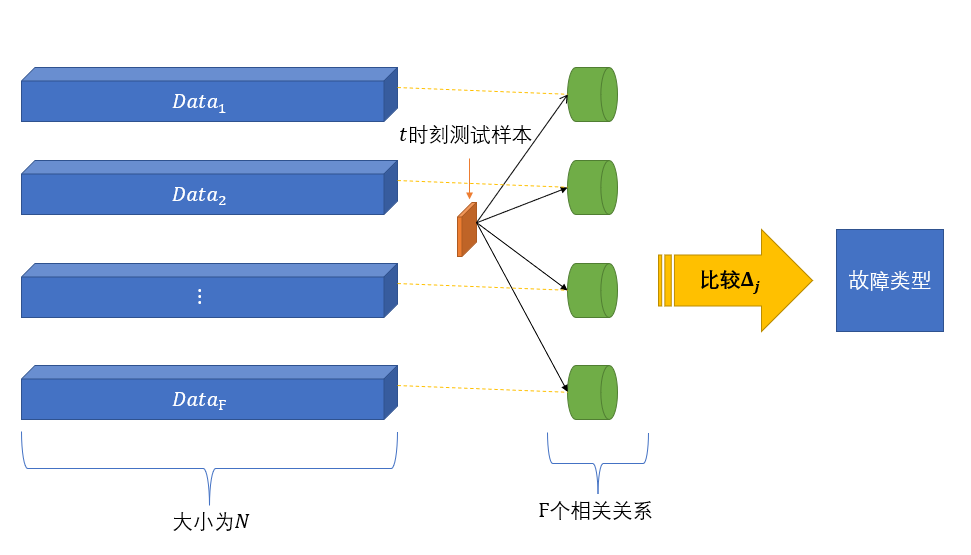
\includegraphics[width=1.0\textwidth]{figure2} %插入图片,[]中设置图片大小,{}中是图片文件名
	\caption{故障辨识框架} %最终文档中希望显示的图片标题
	\label{Fig.main1} %用于文内引用的标签
\end{figure}
\subsection{Further discussion}
前面讨论了最基础的算法的思想,CCA利用过去$\digamma$个故障的$N$个数据构造残差产生器,然后用测试样本依次经过$\digamma$个残差产生器,再通过计算判别式识别出样本的类型。但算法仍然有几个地方不够完善,下面依次进行讨论。
\begin{itemize}
	\item 故障库的数量如何确定?
	\item 故障库如何更新?
	\item 如何改进判别式,使之更加精确?
	\item 如何弱化随机因素在故障辨识中的作用?
	\item 如何辨识新型故障?
	\item $\ldots$
\end{itemize}
\subsubsection{Medium Sample Strategy}
用于构造残差产生器的故障库的大小$N$是越大越好还是越小越好呢?直观上看,$N$越大,(5)式产生的投影向量越稳定,这种情况的稳定是针对整段序列的稳定,而测试样本可以认为位于序列的末端,很有可能序列末端的一小段数据的相关关系和序列开头、中间的发生了一些偏移,这段偏移将影响最终故障辨识的效果。因此需要减小$N$的大小,但$N$过于小容易导致随机因素的干扰变强,也会影响故障辨识的效果。$N$的确定需要根据实验的结果来定,不宜过大也不宜过小,总的原则是:
\begin{itemize}
	\item $N$不能太大,以至于包括测试数据在内的尾端数据与整个故障库相关关系相差太大
	\item $N$不能太小,以至于凸显了随机因素的影响,计算出不稳定的相关关系
\end{itemize}
\begin{figure}[H] %H为当前位置,!htb为忽略美学标准,htbp为浮动图形
	\centering %图片居中
	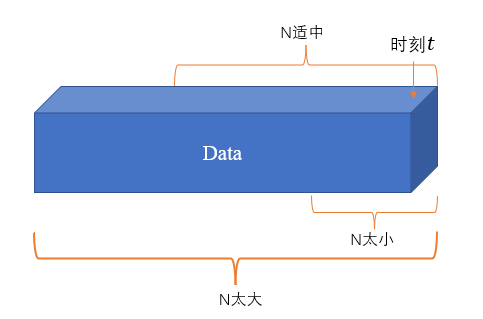
\includegraphics[width=0.7\textwidth]{data} %插入图片,[]中设置图片大小,{}中是图片文件名
	\caption{数据库大小决策} %最终文档中希望显示的图片标题
	\label{Fig.main2} %用于文内引用的标签
\end{figure}
\subsubsection{Updata The Data Step By Step}
1.3.1讨论了中等样本策略,选取合适的$N$能够产生较好的辨识效果。实际进行故障辨识时,我们准备了$\digamma$种故障过去$t-N,\ldots,t-1$采样时刻的数据去识别$t$时刻的样本,这个识别精度一般会达到比较高的水平。
那么下一时刻的样本过来之后,数据库需要更新吗?如何更新呢?显然,随着时间的推移,故障库计算得到的相关关系可能和系统当前采样数据的相关关系发生偏移,尽管偏移可能不大,但是还是会影响到故障辨识。对此,我们采取的策略是利用上一次辨识的结果,将其加入到对应的故障库中,剔除掉故障库最开始的那个数据,以这种方式完成故障库的更新,再进行下一次的辨识。
\begin{figure}[H] %H为当前位置,!htb为忽略美学标准,htbp为浮动图形
	\centering %图片居中
	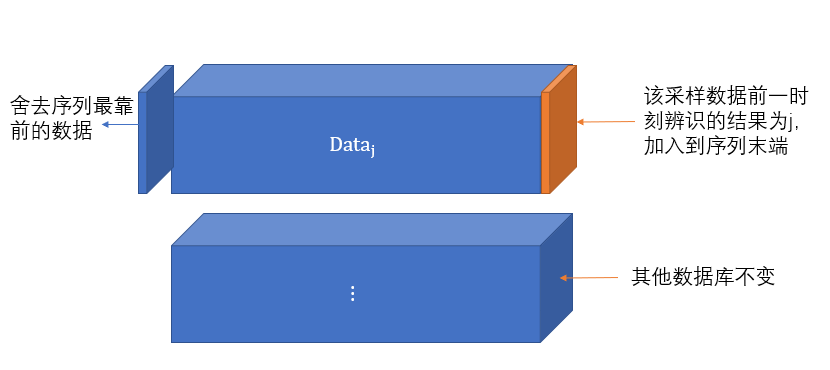
\includegraphics[width=1.0\textwidth]{figure4} %插入图片,[]中设置图片大小,{}中是图片文件名
	\caption{更新数据库} %最终文档中希望显示的图片标题
	\label{Fig.main3} %用于文内引用的标签
\end{figure}
至此,我们给出了数据库的更新方式,另一个显然的问题就是,故障辨识的精度并不是百分百的,那么故障库的更新就会有问题,会掺进并不属于本故障的数据。精度如何变化,有待实验验证。
\subsubsection{
	More Types of Discriminants}
式(15)给出了最简单的一种故障识别的判别式,实际上不同位置的残差地位不同,显然位序为1的残差($i=1$)是由第一对相关关系产生的,这对相关关系对应的相关系数一般非常大,接近于1,由这对相关关系产生的残差比其他相关关系产生的残差更稳定地接近0,我们需要用加权系数为各个相关关系赋不同的重视程度。
设权系数为$\omega_1,\omega_2,\ldots,\omega_s$,定义如下的判别式
\begin{equation}
	\Delta_j' = \sum_{i=1}^{s}\omega_s\left|\boldsymbol{\Sigma}_{u_j}^{-\frac{1}{2}}\boldsymbol{\gamma}_{i,j}\boldsymbol{u_{test}(t)}-\rho_{i,j}\boldsymbol{\Sigma}_{y_j}^{-\frac{1}{2}}\boldsymbol{\lambda}_{i,j}\boldsymbol{y_{test}(t)}\right|
\end{equation}
判别式最大的那个序号即为故障类型
\begin{equation}
	\boldsymbol{type\ of \ fault} = \min \limits_{j} \Delta_j'
\end{equation}
\begin{shaded}
	判别式的种类很多,目前式(14)和式(21)给出了两种判别式,还有其他很多,但总的原则是尽可能考虑各方面的因素,平衡各个因素的影响,最终实现更好的辨识效果。什么是更好的判别式,需要由下面的实验验证。
\end{shaded}
\subsubsection{
	inertia factor}
为了弱化随机因素在故障识别中的作用,增强故障识别的鲁棒性,在此设计一种依照概率的故障转移算法。
算法描述如下:
用$p(t)\in\left[ 0,1\right] $表示切换概率,指的是当$t$时刻故障识别结果和$t-1$时刻不同时,不会立即改变识别结果,而是以$p(t)$的概率切换识别结果,以次弱化随机因素的影响。$t$时刻产生一个$\left[ 0,1\right] $的服从均匀分布的随机数$s(t)$,
\begin{equation}
	\begin{cases}
		\text{不保持}t-1\text{时刻的识别结果} &s(t)\geq p(t)\\
		\text{保持$t-1$时刻的识别结果} &s(t)< p(t)
	\end{cases}
\end{equation}
\begin{shaded}
	{这里的操作步骤是,如果$t$时刻产生的随机数大于切换概率,那表示视$t$时刻实际的辨识结果为真,并不是随机因素,应予以采纳。如果$t$时刻产生的随机数小于切换概率,那表示视$t$时刻实际的辨识结果为随机误差,不予采纳,保持$t-1$时刻的辨识结果}。该理念借助物理学中惯性的概念,因此称为“惯性因子”(inertia factor).
\end{shaded}
惯性因子$p(t)$初始值为0,表示算法开始时不受该因子的影响。该因子下界为0,上界设为$\xi$,每次更新$p(t)$的正补偿设为$\delta_+$,负的步长设为$\delta_-$。
根据(15)式,得出$p(t)$的更新步骤为:
\begin{equation}
	\begin{cases}
		p(t)  = p(t-1)+\delta_+ &\min \limits_{j}\Delta_j(t-1) = \min \limits_{j}\Delta_j(t-2),j = 1,\ldots \digamma\\
		p(t)  = p(t-1)-\delta_- &\min \limits_{j}\Delta_j(t-1)\neq \min \limits_{j}\Delta_j(t-2), j= 1,\ldots,\digamma\\
		p(t) = \xi &p(t)>\xi\\
		p(t) = 0 &p(t)<0
	\end{cases}
\end{equation}
\begin{shaded}
	\begin{itemize}
		\item 式(20)表述了惯性因子$p(t)$的更新方式,该组方程式中前两个表述了当两个时刻的辨识结果相同的时候,再下一个时刻的惯性因子会增大,这表示了有更大的概率保持上次识别结果,这在连续一段辨识结果都相同相同,突然出现一个异常的辨识结果时,有非常明显的效果,这就是“惯性”非常大的体现。
		\item 
		当两个时刻的辨识结果不同的时候,再下一个时刻的惯性因子会减小,这表示有更小的概率保持上次识别结果,换言之,“惯性”变小了
	\end{itemize}
\end{shaded}
\subsubsection{New type of Fault}
系统过去存储了$\digamma$种故障,但有一定的可能会出现新型故障,这种新型故障也能通过计算判别式来找到一个故障类型,但从数据特征上讲,与数据库中的故障有所区别。为此,设计如下的算法检验测试样本是否为新型故障:
单个测试样本有随机性因素的影响,为此需要一段连续的测试样本。假设有一段测试样本$\left[\begin{array}{c}
	\boldsymbol{U_{test}}\\
	\boldsymbol{Y_{test}}
\end{array}\right]=\left[\begin{array}{cccc}
	\boldsymbol{u}_{test}(t_0)& \boldsymbol{u}_{test}(t_0+1) &\ldots  & \boldsymbol{u}_{test}(t_0+n-1) \\
	\boldsymbol{y}_{test}(t_0)& \boldsymbol{y}_{test}(t_0+1) &\ldots  & \boldsymbol{y}_{test}(t_0+n-1)
\end{array}\right]$,经判别式计算得到故障类型为$j$型故障(大部分为$j$型故障),在进行故障辨识时已经计算了这段序列的残差:
\begin{equation}
	\begin{cases}
		r_{i,test}(t) = \boldsymbol{\Sigma}_{u_{j}}^{-\frac{1}{2}}\boldsymbol{\gamma}_{i,j}\boldsymbol{u}_{test}(t)-\boldsymbol{\Sigma}_{y_{j}}^{-\frac{1}{2}}\boldsymbol{\lambda}_{i,j}\boldsymbol{y}_{test}(t)\\
		i = 1,\ldots,s\quad t = t_0,\ldots,t_0+n-1
	\end{cases}
\end{equation}
这段序列的判别式为$\Delta_j'(t) = \sum_{i=1}^{s}\omega_s\left|\boldsymbol{\Sigma}_{u_j}^{-\frac{1}{2}}\boldsymbol{\gamma}_{i,j}\boldsymbol{u_{test}(t)}-\rho_{i,j}\boldsymbol{\Sigma}_{y_j}^{-\frac{1}{2}}\boldsymbol{\lambda}_{i,j}\boldsymbol{y_{test}(t)}\right|,t = t_0,\ldots,t_0+n-1$,设判断新型故障的判别式为
\begin{equation}
	\Delta_{new} = \frac{1}{n}\sum_{t=1}^{n}\Delta_j' 
\end{equation}
\begin{shaded}
	{\textbf{注意}:产生相关关系投影向量$\left\langle \boldsymbol{\Sigma}_{u_{j}}^{-\frac{1}{2}}\boldsymbol{\gamma}_{i,j},\boldsymbol{\Sigma}_{y_{j}}^{-\frac{1}{2}}\boldsymbol{\lambda}_{i,j}\right\rangle $的数据库是随时间步更新的。}
\end{shaded}
式(21)表达了测试样本判别式的平均大小,一般来说,如果该测试样本属于某种故障库中的一员,则该判别式应该与此故障库的判别式相近,据此可以判断是否为新型故障
\begin{equation}
	\begin{cases}
		new\ type &\Delta_{new}>\Delta_{\alpha}
		\\
		old\ type &\Delta_{new}\leq\Delta_{\alpha}
	\end{cases}
\end{equation}
$\Delta_{\alpha}$表示区分新旧类型故障的临界点,与不同的故障类型有关,需要从故障库中学习得到。
\section{Experiment}
本章展示实验结果,验证前面所述的理论。实验用到的例子是$4\times 4$的数值例子。
\begin{figure}[H] %H为当前位置,!htb为忽略美学标准,htbp为浮动图形
	\centering %图片居中
	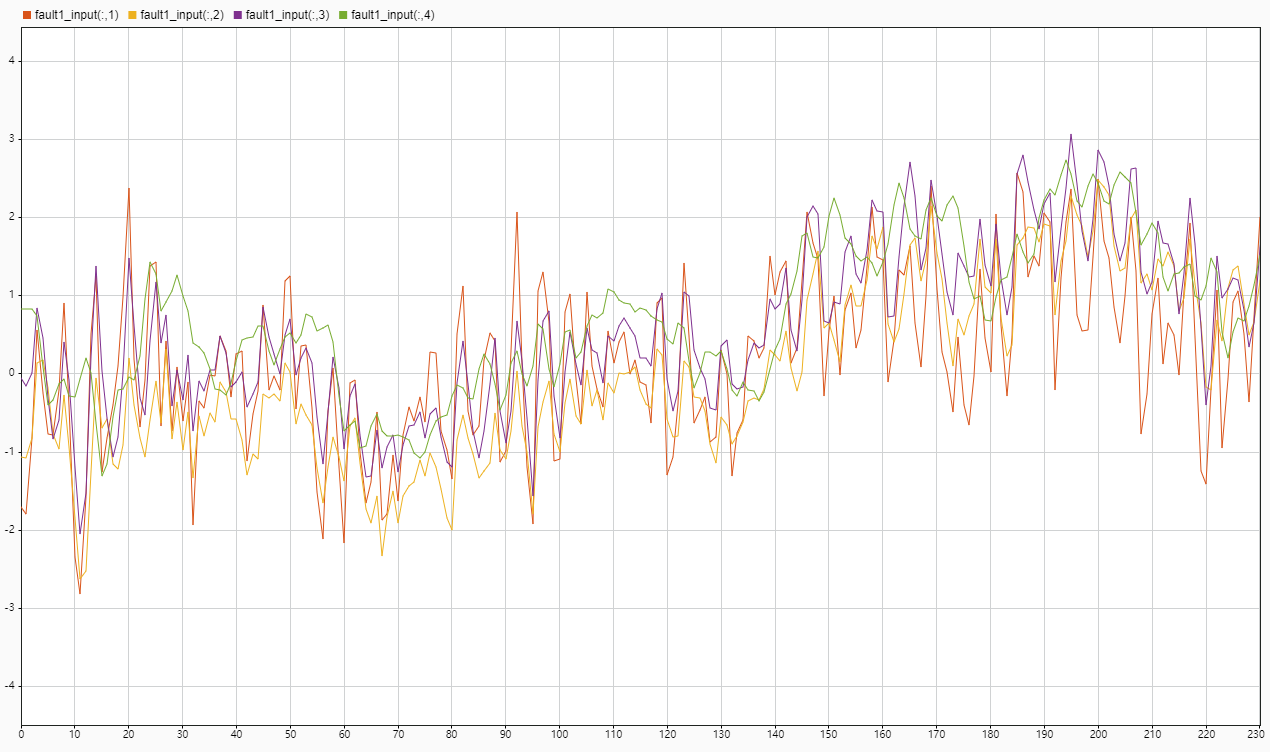
\includegraphics[width=1.0\textwidth]{fault1_input} %插入图片,[]中设置图片大小,{}中是图片文件名
	\caption{故障1的4个输入(部分数据)} %最终文档中希望显示的图片标题
	\label{Fig.main2} %用于文内引用的标签
\end{figure}
\begin{figure}[H] %H为当前位置,!htb为忽略美学标准,htbp为浮动图形
	\centering %图片居中
	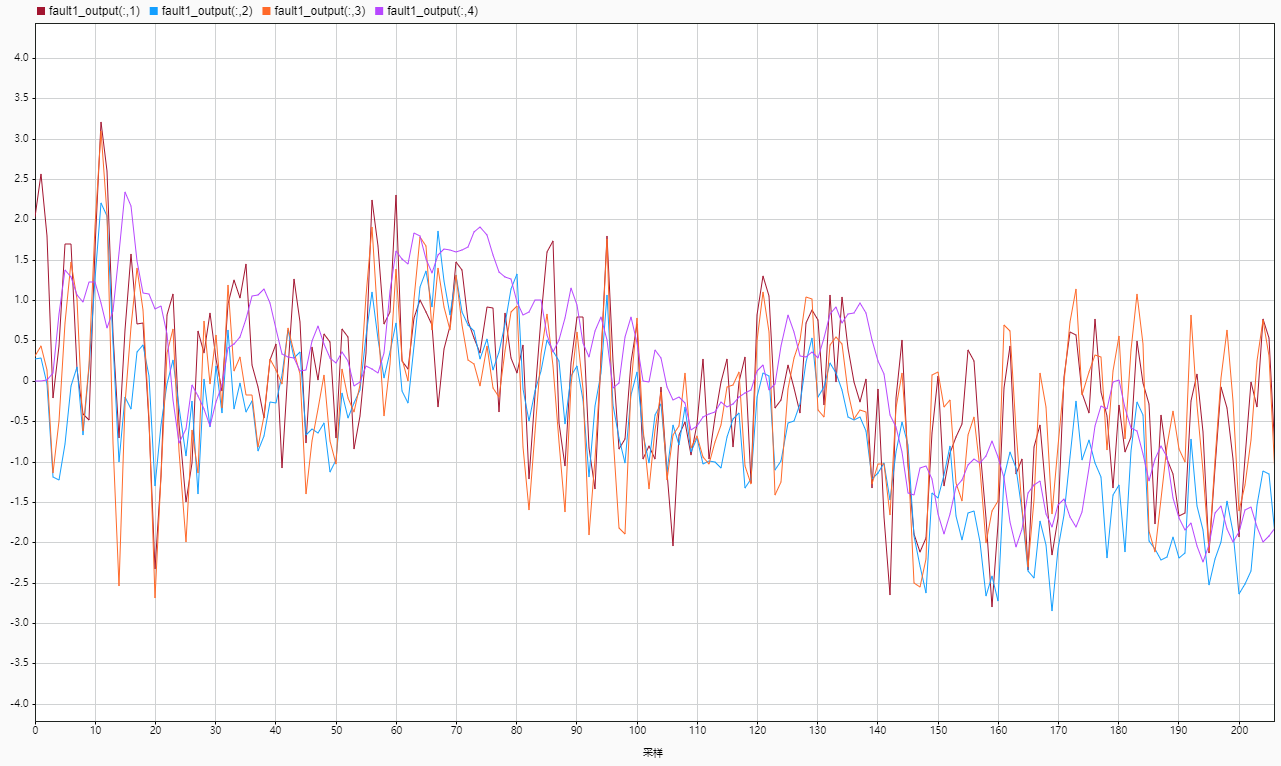
\includegraphics[width=1.0\textwidth]{fault1_output} %插入图片,[]中设置图片大小,{}中是图片文件名
	\caption{故障1的4个输出(部分数据)} %最终文档中希望显示的图片标题
	\label{Fig.main2} %用于文内引用的标签
\end{figure}
\begin{figure}[H] %H为当前位置,!htb为忽略美学标准,htbp为浮动图形
	\centering %图片居中
	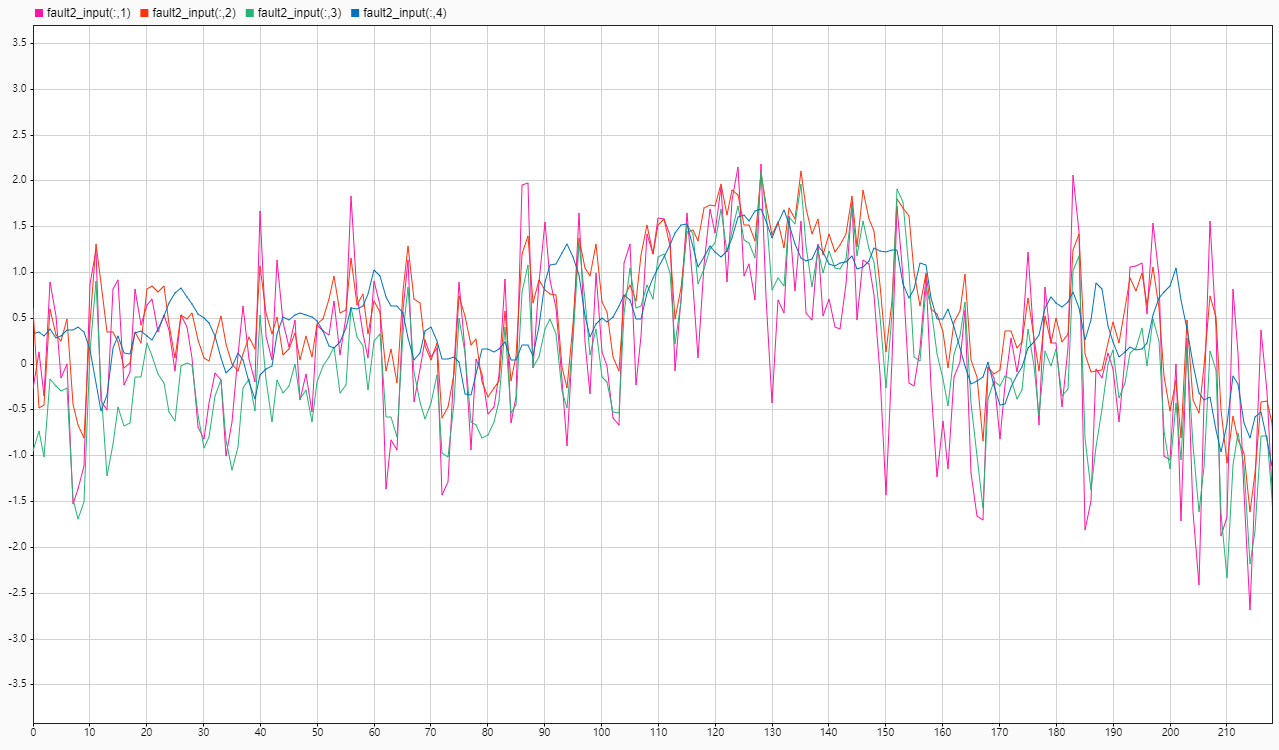
\includegraphics[width=1.0\textwidth]{fault2_input} %插入图片,[]中设置图片大小,{}中是图片文件名
	\caption{故障2的4个输入(部分数据)} %最终文档中希望显示的图片标题
	\label{Fig.main2} %用于文内引用的标签
\end{figure}
\begin{figure}[H] %H为当前位置,!htb为忽略美学标准,htbp为浮动图形
	\centering %图片居中
	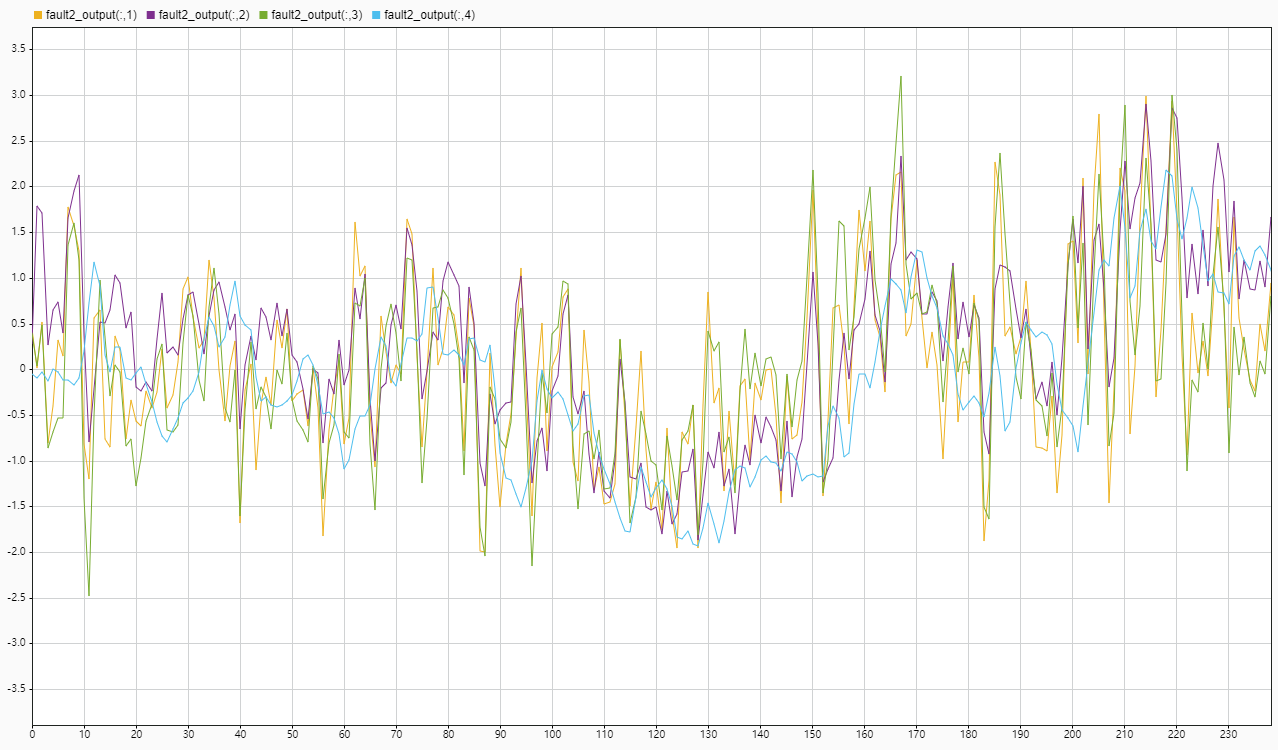
\includegraphics[width=1.0\textwidth]{fault2_output} %插入图片,[]中设置图片大小,{}中是图片文件名
	\caption{故障2的4个输出(部分数据)} %最终文档中希望显示的图片标题
	\label{Fig.main2} %用于文内引用的标签
\end{figure}
\begin{figure}[H] %H为当前位置,!htb为忽略美学标准,htbp为浮动图形
	\centering %图片居中
	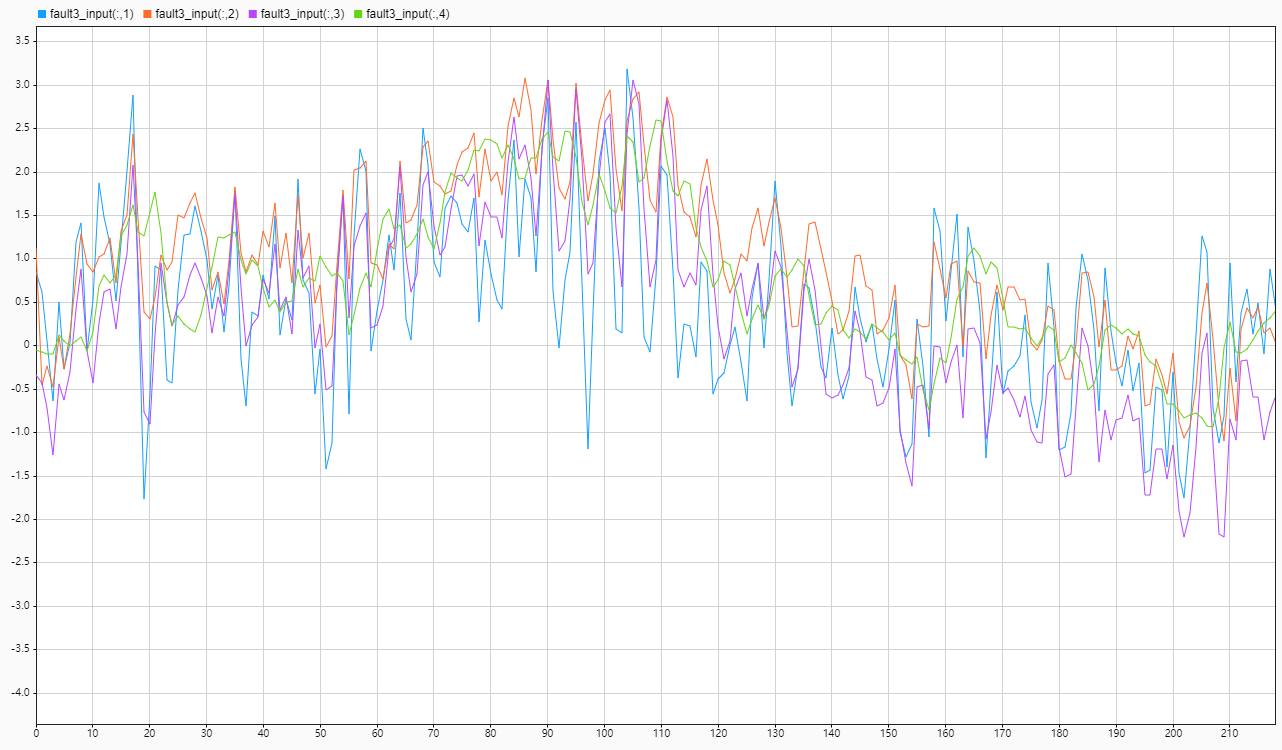
\includegraphics[width=1.0\textwidth]{fault3_input} %插入图片,[]中设置图片大小,{}中是图片文件名
	\caption{故障3的4个输入(部分数据)} %最终文档中希望显示的图片标题
	\label{Fig.main2} %用于文内引用的标签
\end{figure}
\begin{figure}[H] %H为当前位置,!htb为忽略美学标准,htbp为浮动图形
	\centering %图片居中
	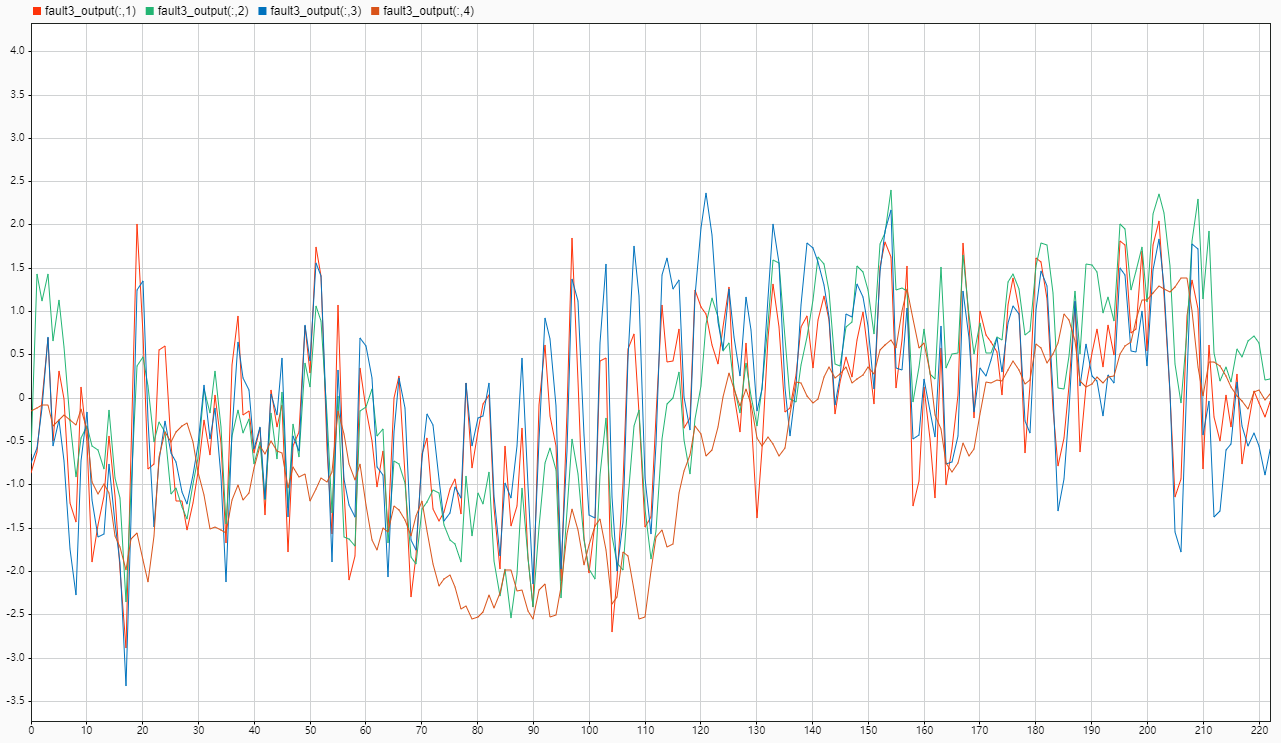
\includegraphics[width=1.0\textwidth]{fault3_output} %插入图片,[]中设置图片大小,{}中是图片文件名
	\caption{故障3的4个输出(部分数据)} %最终文档中希望显示的图片标题
	\label{Fig.main2} %用于文内引用的标签
\end{figure}
\begin{figure}[H] %H为当前位置,!htb为忽略美学标准,htbp为浮动图形
	\centering %图片居中
	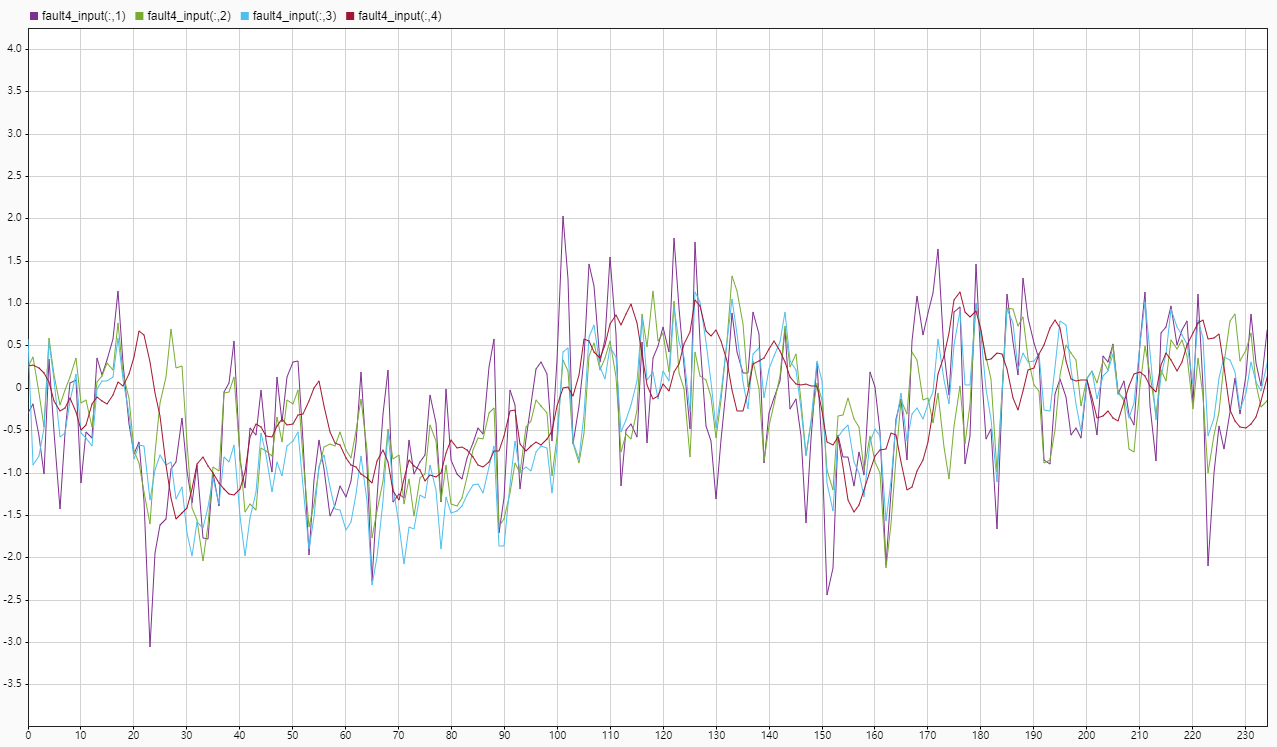
\includegraphics[width=1.0\textwidth]{fault4_input} %插入图片,[]中设置图片大小,{}中是图片文件名
	\caption{故障4的4个输入(部分数据)} %最终文档中希望显示的图片标题
	\label{Fig.main2} %用于文内引用的标签
\end{figure}
\begin{figure}[H] %H为当前位置,!htb为忽略美学标准,htbp为浮动图形
	\centering %图片居中
	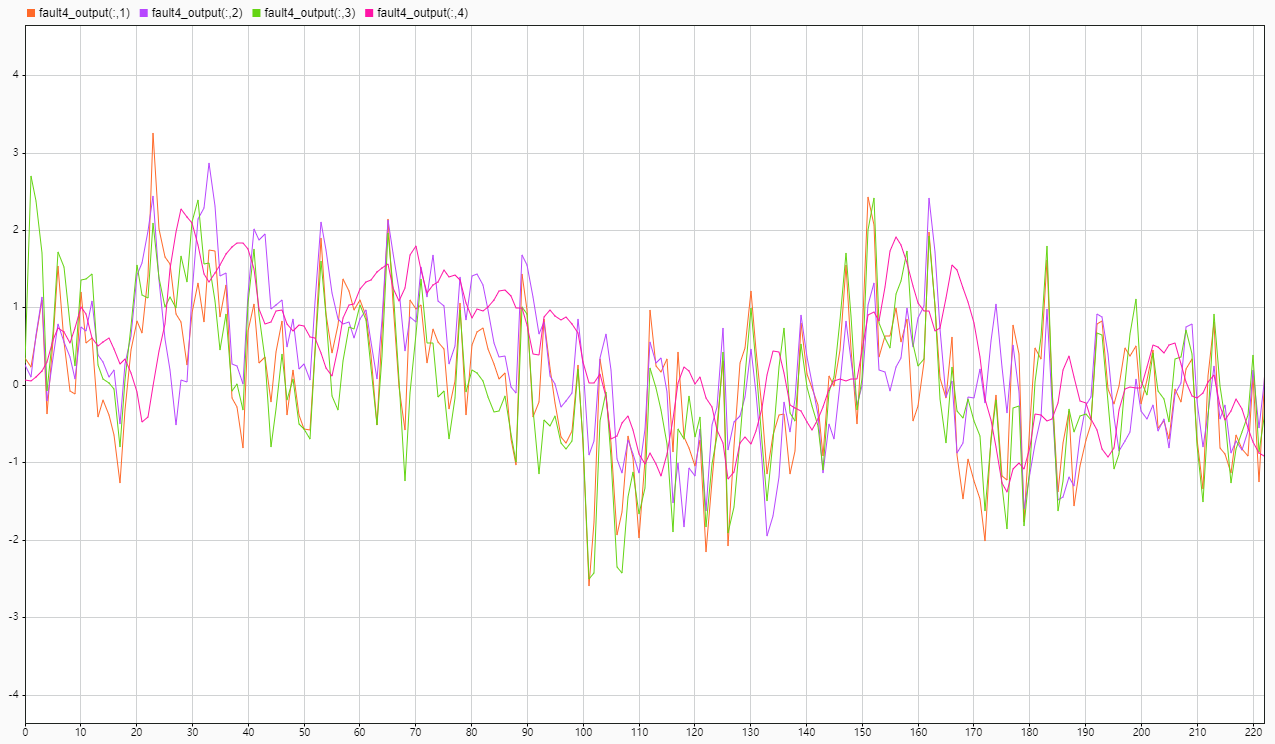
\includegraphics[width=1.0\textwidth]{fault4_output} %插入图片,[]中设置图片大小,{}中是图片文件名
	\caption{故障4的4个输出(部分数据)} %最终文档中希望显示的图片标题
	\label{Fig.main2} %用于文内引用的标签
\end{figure}
\subsection{实验一:探究故障库的大小对故障辨识的影响}
本实验探究1.3.1节提出的如何选择合适的样本大小。本次实验不更新数据库,以及采用的判别式是最原始的判别式。
\begin{shaded}
	注意:本次实验不更新数据库
\end{shaded}
\subsubsection{$N=100$}
取数据库中$901:1000$时刻的数据作为数据库,$1001:1100$时刻的数据作为测试样本。
\begin{figure}[H]
	\centering  %图片全局居中
	\subfigure[故障1]{
		\label{Fig.sub.1}
		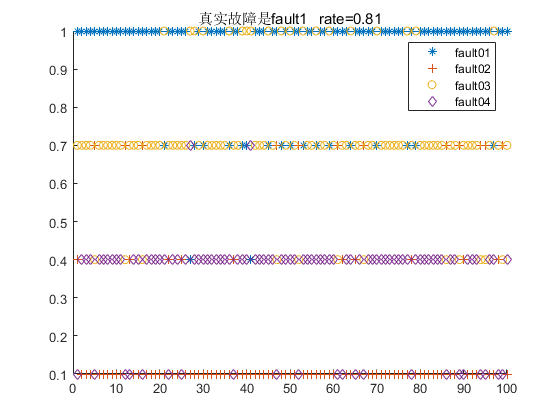
\includegraphics[width=0.45\textwidth]{exp1_1}}
	\subfigure[故障2]{
		\label{Fig.sub.2}
		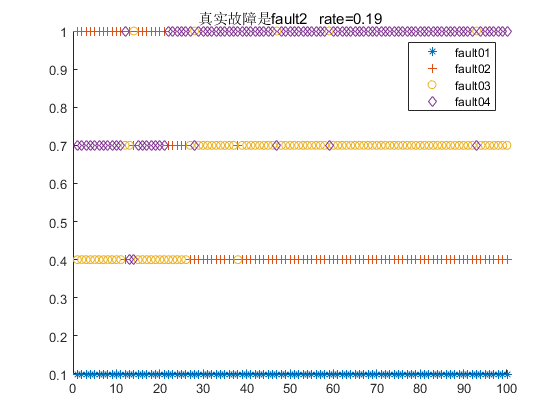
\includegraphics[width=0.45\textwidth]{exp1_2}}
	\subfigure[故障3]{
		\label{Fig.sub.3}
		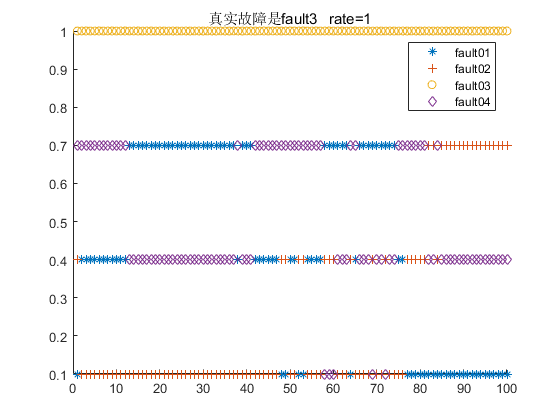
\includegraphics[width=0.45\textwidth]{exp1_3}}
	\subfigure[故障4]{
		\label{Fig.sub.4}
		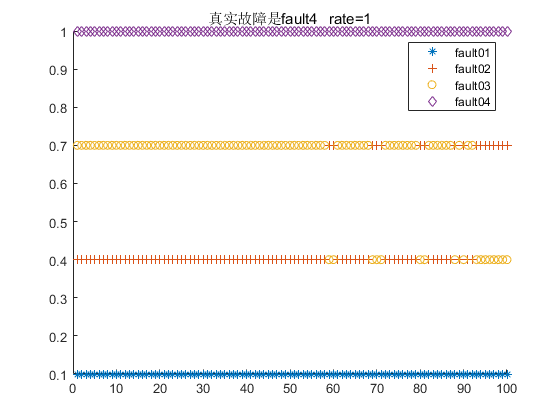
\includegraphics[width=0.45\textwidth]{exp1_4}}
	\caption{$N=100$时故障辨识效果}
	\label{Fig.main}
\end{figure}
注意到故障2识别率较低,原因有很多,可能是故障库N选取不对,也可能是判别式需要更改,还有可能是故障库没有更新的缘故。
\subsubsection{$N = 500$}
取数据库中$501:1000$时刻的数据作为数据库,$1001:1100$时刻的数据作为测试样本。
\begin{figure}[H]
	\centering  %图片全局居中
	\subfigure[故障1]{
		\label{Fig.sub.1}
		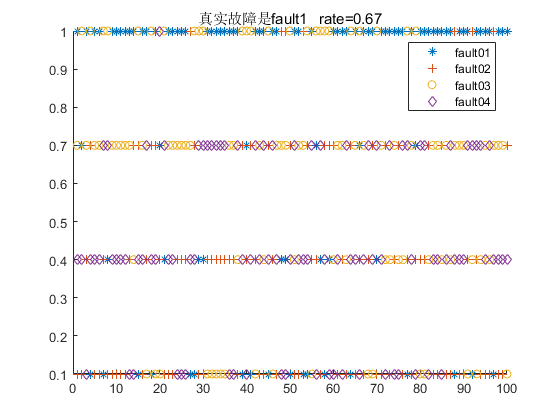
\includegraphics[width=0.45\textwidth]{exp1_5}}
	\subfigure[故障2]{
		\label{Fig.sub.2}
		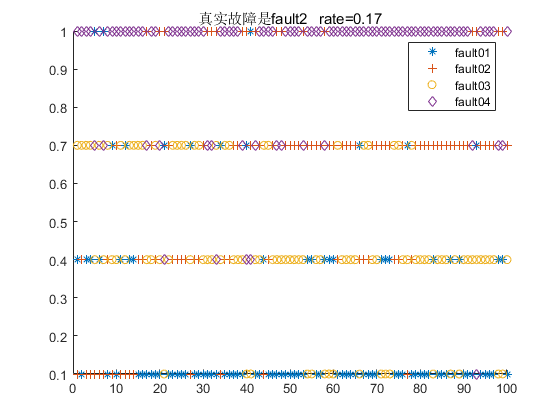
\includegraphics[width=0.45\textwidth]{exp1_6}}
	\subfigure[故障3]{
		\label{Fig.sub.3}
		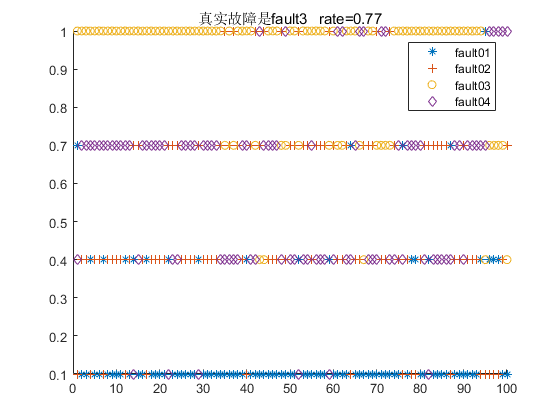
\includegraphics[width=0.45\textwidth]{exp1_7}}
	\subfigure[故障4]{
		\label{Fig.sub.4}
		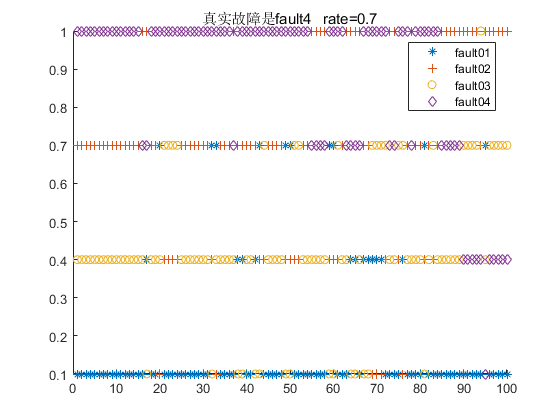
\includegraphics[width=0.45\textwidth]{exp1_8}}
	\caption{$N=500$时故障辨识效果}
	\label{Fig.main}
\end{figure}
可以看到,4种故障辨识的效果相对$N=100$时有明显下降。
\subsubsection{$N = 1000$}
取数据库中$1:1000$时刻的数据作为数据库,$1001:1100$时刻的数据作为测试样本。
\begin{figure}[H]
	\centering  %图片全局居中
	\subfigure[故障1]{
		\label{Fig.sub.1}
		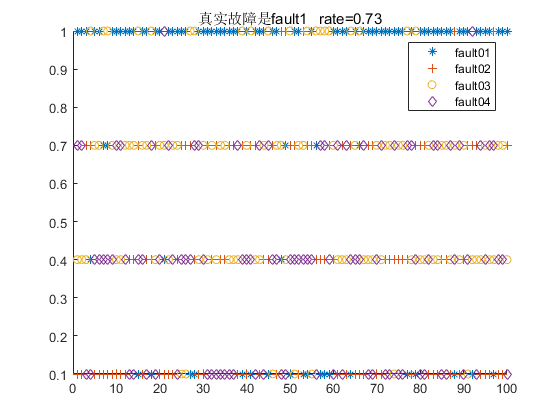
\includegraphics[width=0.45\textwidth]{exp1_9}}
	\subfigure[故障2]{
		\label{Fig.sub.2}
		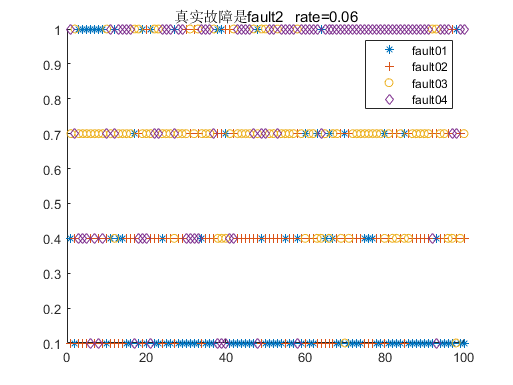
\includegraphics[width=0.45\textwidth]{exp1_10}}
	\subfigure[故障3]{
		\label{Fig.sub.3}
		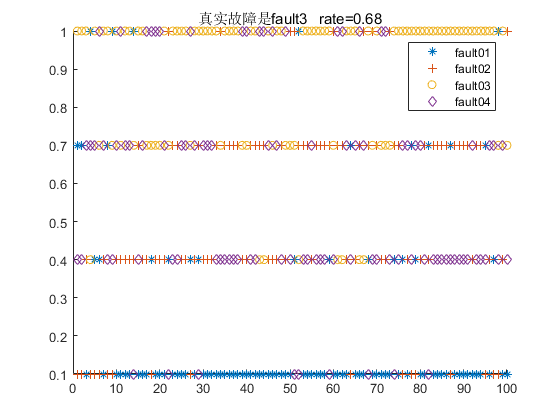
\includegraphics[width=0.45\textwidth]{exp1_11}}
	\subfigure[故障4]{
		\label{Fig.sub.4}
		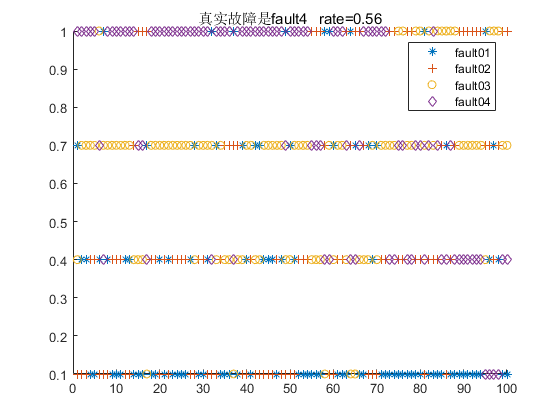
\includegraphics[width=0.45\textwidth]{exp1_12}}
	\caption{$N=1000$时故障辨识效果}
	\label{Fig.main}
\end{figure}
实验总结:样本个数确实能够影响故障辨识的效果,要寻找最优的$N$的值需要遍历测试,本次实验最优的$N$的值在100附近。
\subsection{实验二:探究故障库更新对故障辨识的影响}
\begin{shaded}
	本次实验采用的故障库大小为$N=100$
\end{shaded}
用13.2节提出的方式进行故障库数据的更新,效果如下:
\begin{figure}[H]
	\centering  %图片全局居中
	\subfigure[故障1]{
		\label{Fig.sub.1}
		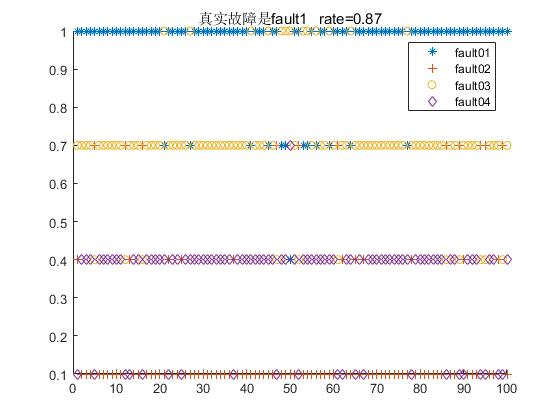
\includegraphics[width=0.45\textwidth]{exp2_1}}
	\subfigure[故障2]{
		\label{Fig.sub.2}
		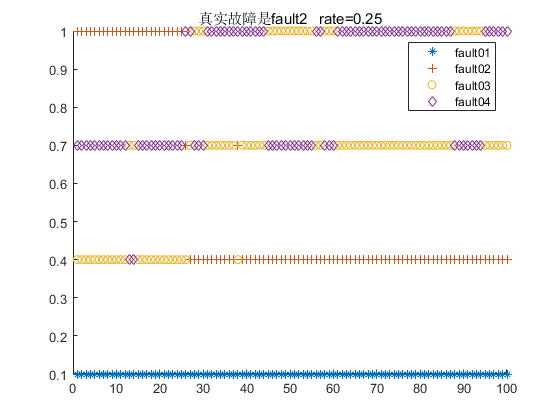
\includegraphics[width=0.45\textwidth]{exp2_2}}
	\subfigure[故障3]{
		\label{Fig.sub.3}
		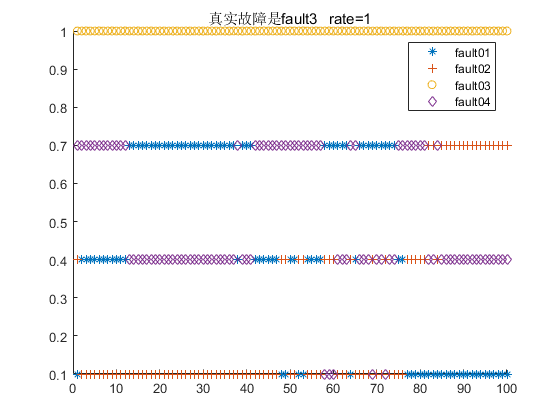
\includegraphics[width=0.45\textwidth]{exp2_3}}
	\subfigure[故障4]{
		\label{Fig.sub.4}
		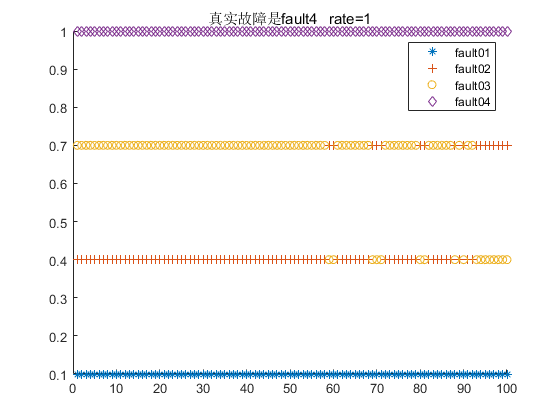
\includegraphics[width=0.45\textwidth]{exp2_4}}
	\caption{更新故障库时的辨识效果}
	\label{Fig.main}
\end{figure}
实验总结:相较于实验$\boldsymbol{2.1.1}$,故障1的识别正确率提高了4个百分点,故障2提高了6个不百分点,故障3和故障4识别精度不变,都为百分之百。
\begin{figure}[H] %H为当前位置,!htb为忽略美学标准,htbp为浮动图形
	\centering %图片居中
	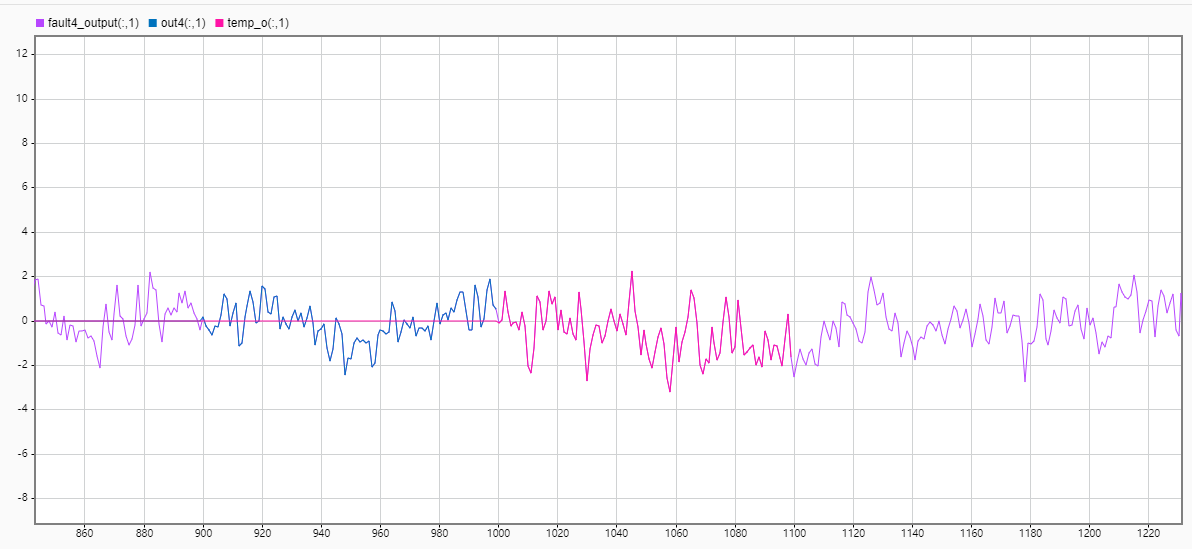
\includegraphics[width=1.0\textwidth]{exp2_5} %插入图片,[]中设置图片大小,{}中是图片文件名
	\caption{故障4的数据库的更新} %最终文档中希望显示的图片标题
	\label{Fig.main2} %用于文内引用的标签
\end{figure}
以故障4为例,因为识别率百分之百,因此每一步识别之后故障库都会更新,最后会形成整体的推移。图中紫色线是采集的数据,蓝色线是作为故障库的数据,红线是最后更新的故障库,会看到和采集数据的1101:1200是重合的。
\subsection{实验三:判别式的精进}
本次实验验证式(21)比式(14)更加精准。$\omega_1,\ldots,\omega_s$分别对应$s$对相关关系,为了增加对前面的相关关系的重视程度,令$\omega_1>\ldots>\omega_s$,凸显出前面位置相关关系的重要性。实验结果显示如下:
\begin{figure}[H]
	\centering  %图片全局居中
	\subfigure[故障1]{
		\label{Fig.sub.1}
		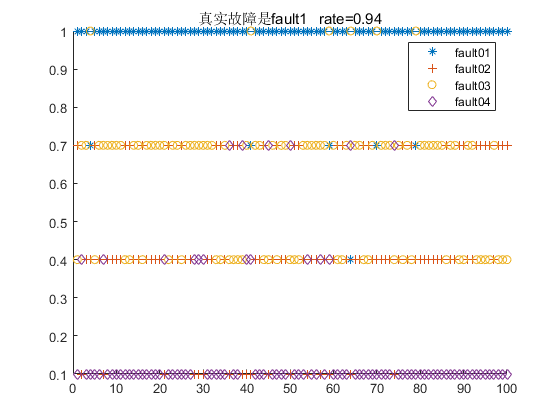
\includegraphics[width=0.45\textwidth]{exp3_1}}
	\subfigure[故障2]{
		\label{Fig.sub.2}
		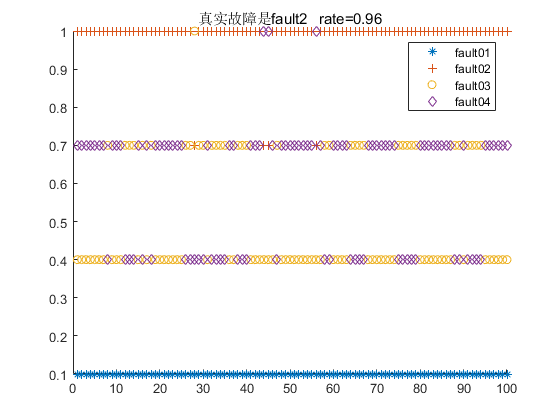
\includegraphics[width=0.45\textwidth]{exp3_2}}
	\subfigure[故障3]{
		\label{Fig.sub.3}
		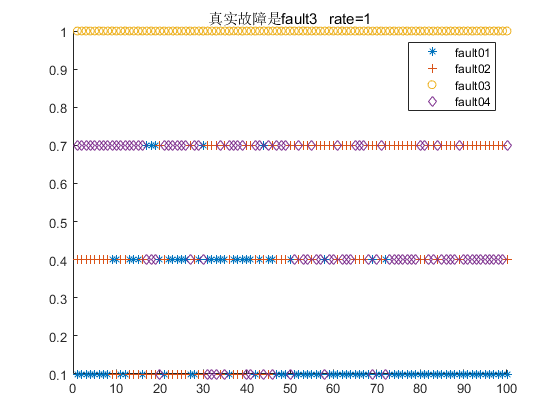
\includegraphics[width=0.45\textwidth]{exp3_3}}
	\subfigure[故障4]{
		\label{Fig.sub.4}
		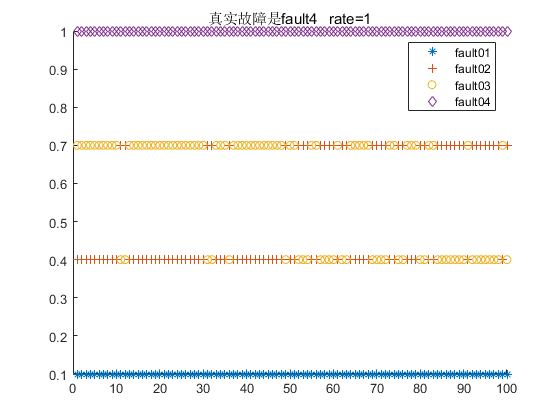
\includegraphics[width=0.45\textwidth]{exp3_4}}
	\caption{改变判别式时的辨识效果}
	\label{Fig.main}
\end{figure}
实验总结:由实验结果可知,故障1的辨识精度小幅提升,故障2的辨识精度大幅提升。
\subsection{实验四:检验惯性因子的效果}
本次实验验证式19描述惯性因子的效果。
\begin{figure}[H]
	\centering  %图片全局居中
	\subfigure[故障1]{
		\label{Fig.sub.1}
		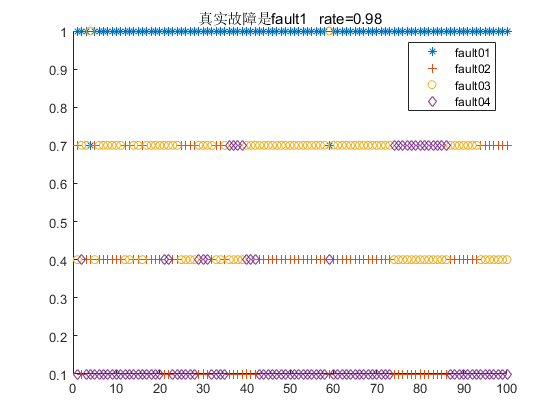
\includegraphics[width=0.45\textwidth]{exp4_1}}
	\subfigure[故障2]{
		\label{Fig.sub.2}
		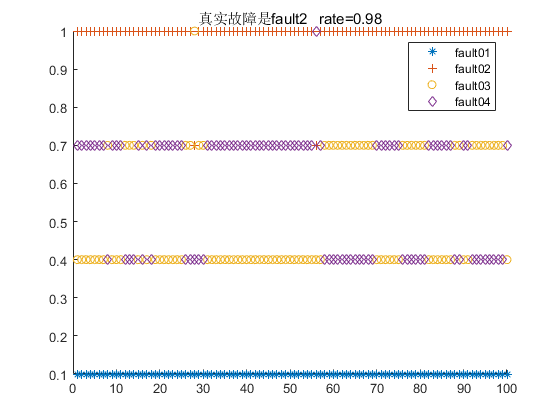
\includegraphics[width=0.45\textwidth]{exp4_2}}
	\subfigure[故障3]{
		\label{Fig.sub.3}
		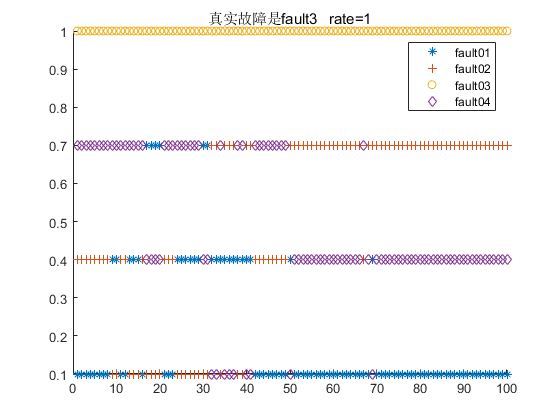
\includegraphics[width=0.45\textwidth]{exp4_3}}
	\subfigure[故障4]{
		\label{Fig.sub.4}
		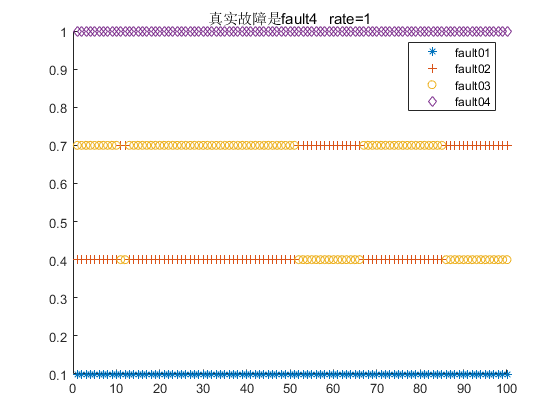
\includegraphics[width=0.45\textwidth]{exp4_4}}
	\caption{增加惯性因子时的辨识效果}
	\label{Fig.main}
\end{figure}
实验总结:增加惯性因子后,在惯性的作用下会消除一些随机性因素的影响,可以观察到故障1的辨识率提高了4个百分点,故障2辨识率提高了2个百分点。总的来说惯性因子对最终的识别效果是锦上添花的,不是决定性的。
\subsubsection{拼接实验}
将故障1和故障3的各50个采样点拼接到一起作为一段序列,进行故障识别。效果如下:
\begin{figure}[H] %H为当前位置,!htb为忽略美学标准,htbp为浮动图形
	\centering %图片居中
	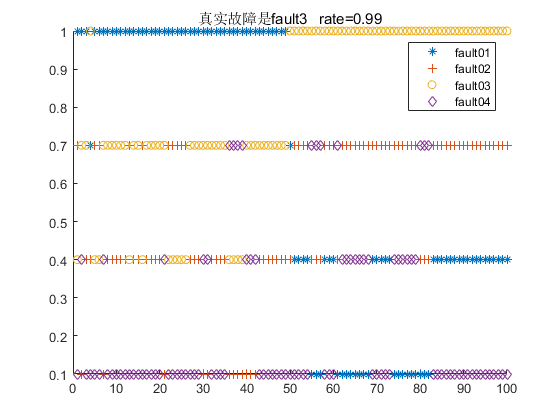
\includegraphics[width=1.0\textwidth]{exp4_5} %插入图片,[]中设置图片大小,{}中是图片文件名
	\caption{拼接后的故障识别效果} %最终文档中希望显示的图片标题
	\label{Fig.main2} %用于文内引用的标签
\end{figure}
\subsection{识别新型故障}
根据式(22),识别新型故障前需要得到$\Delta_{\alpha}$,这个可以从故障库中学习得到。
从仿真中得到5000个采样点,以250为步长,故障库大小为100,测试样本数目为100,测得4个样本各19个$Delta_\alpha$然后从中取最大值作为该故障最终的临界值。
\begin{figure}[H]
	\centering  %图片全局居中
	\subfigure[故障1]{
		\label{Fig.sub.1}
		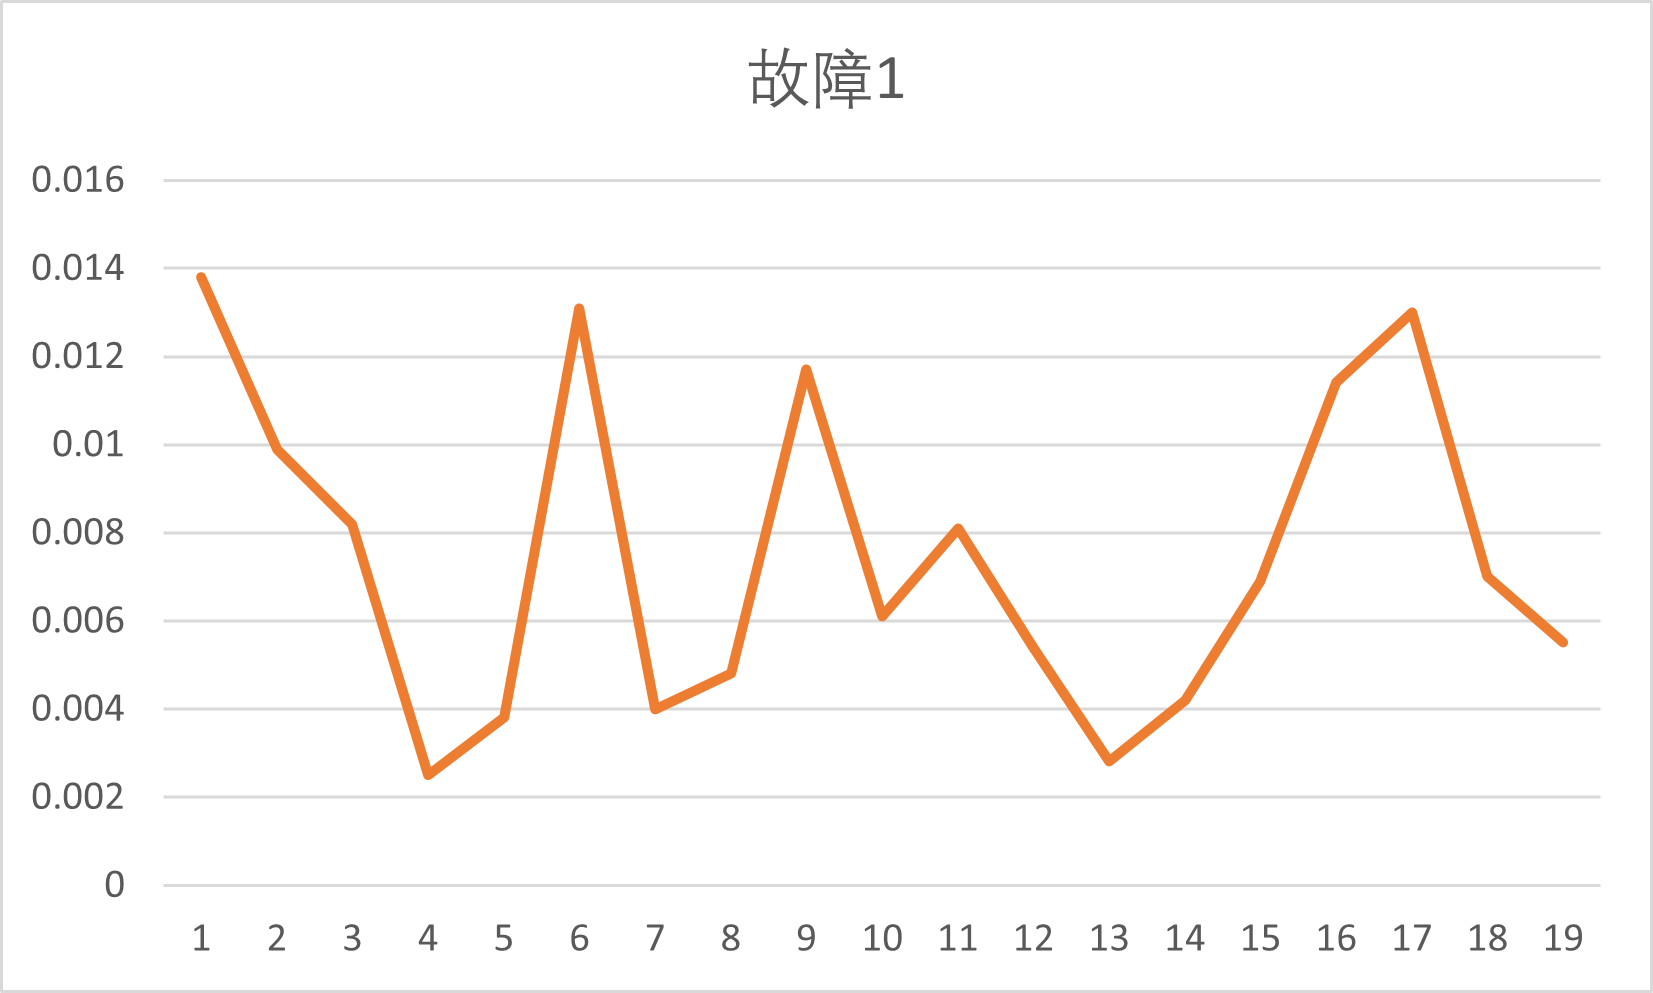
\includegraphics[width=0.45\textwidth]{exp5_2}}
	\subfigure[故障2]{
		\label{Fig.sub.2}
		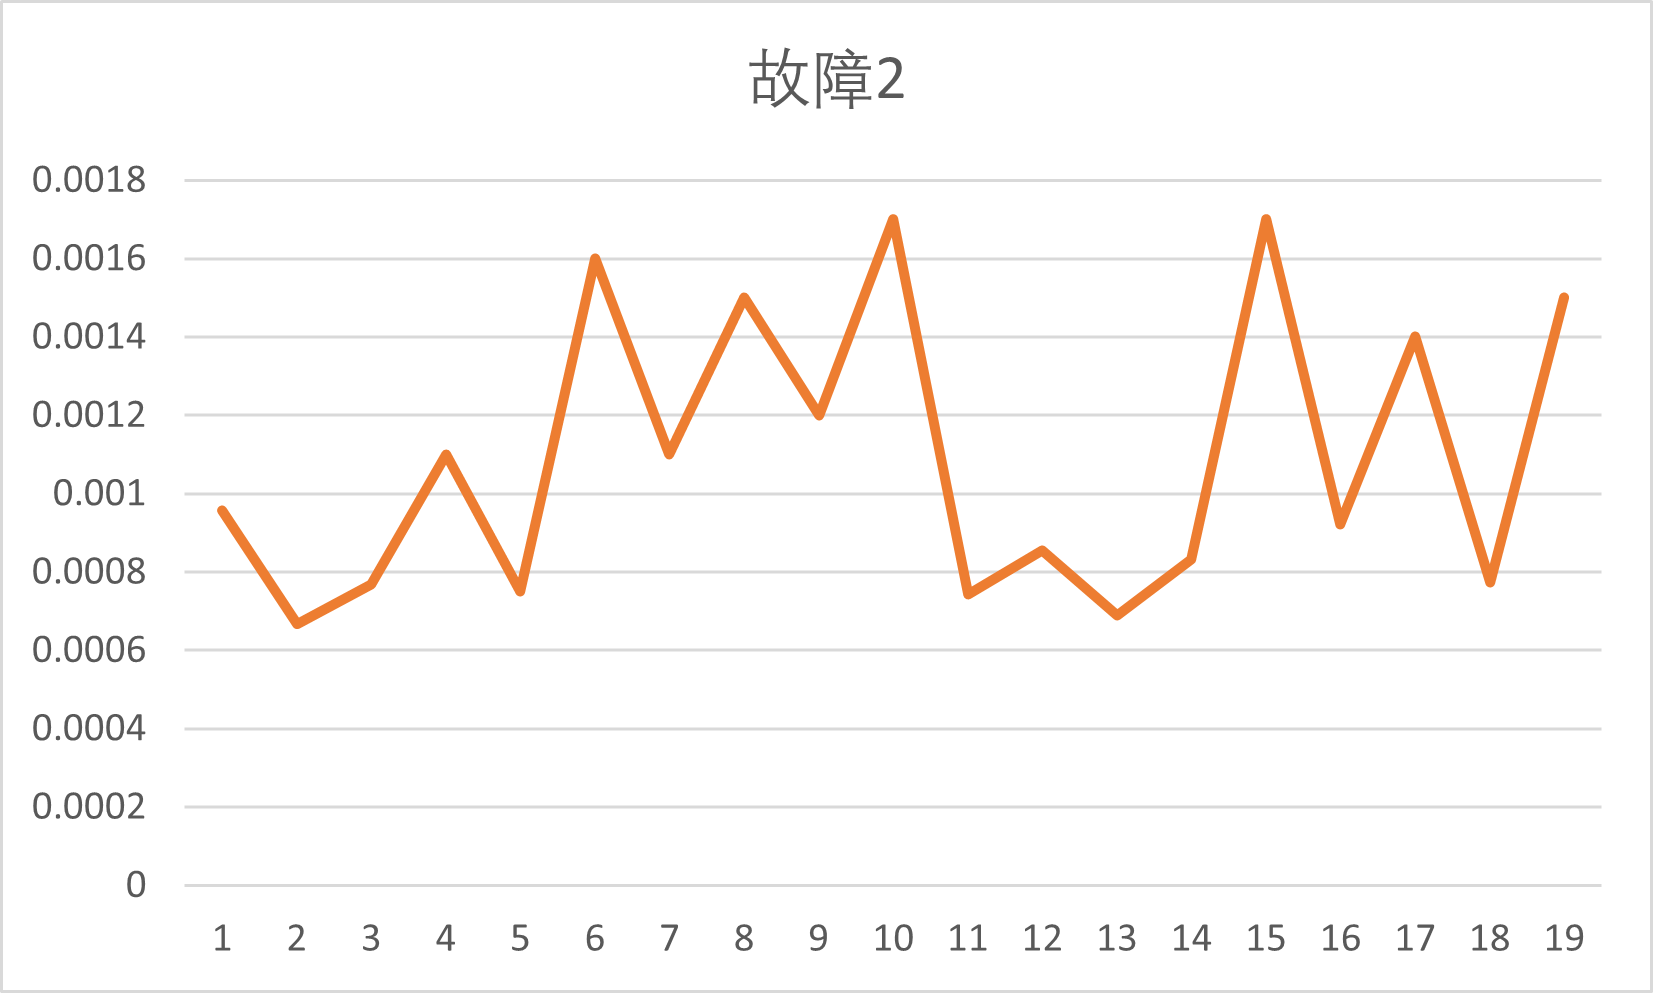
\includegraphics[width=0.45\textwidth]{exp5_3}}
	\subfigure[故障3]{
		\label{Fig.sub.3}
		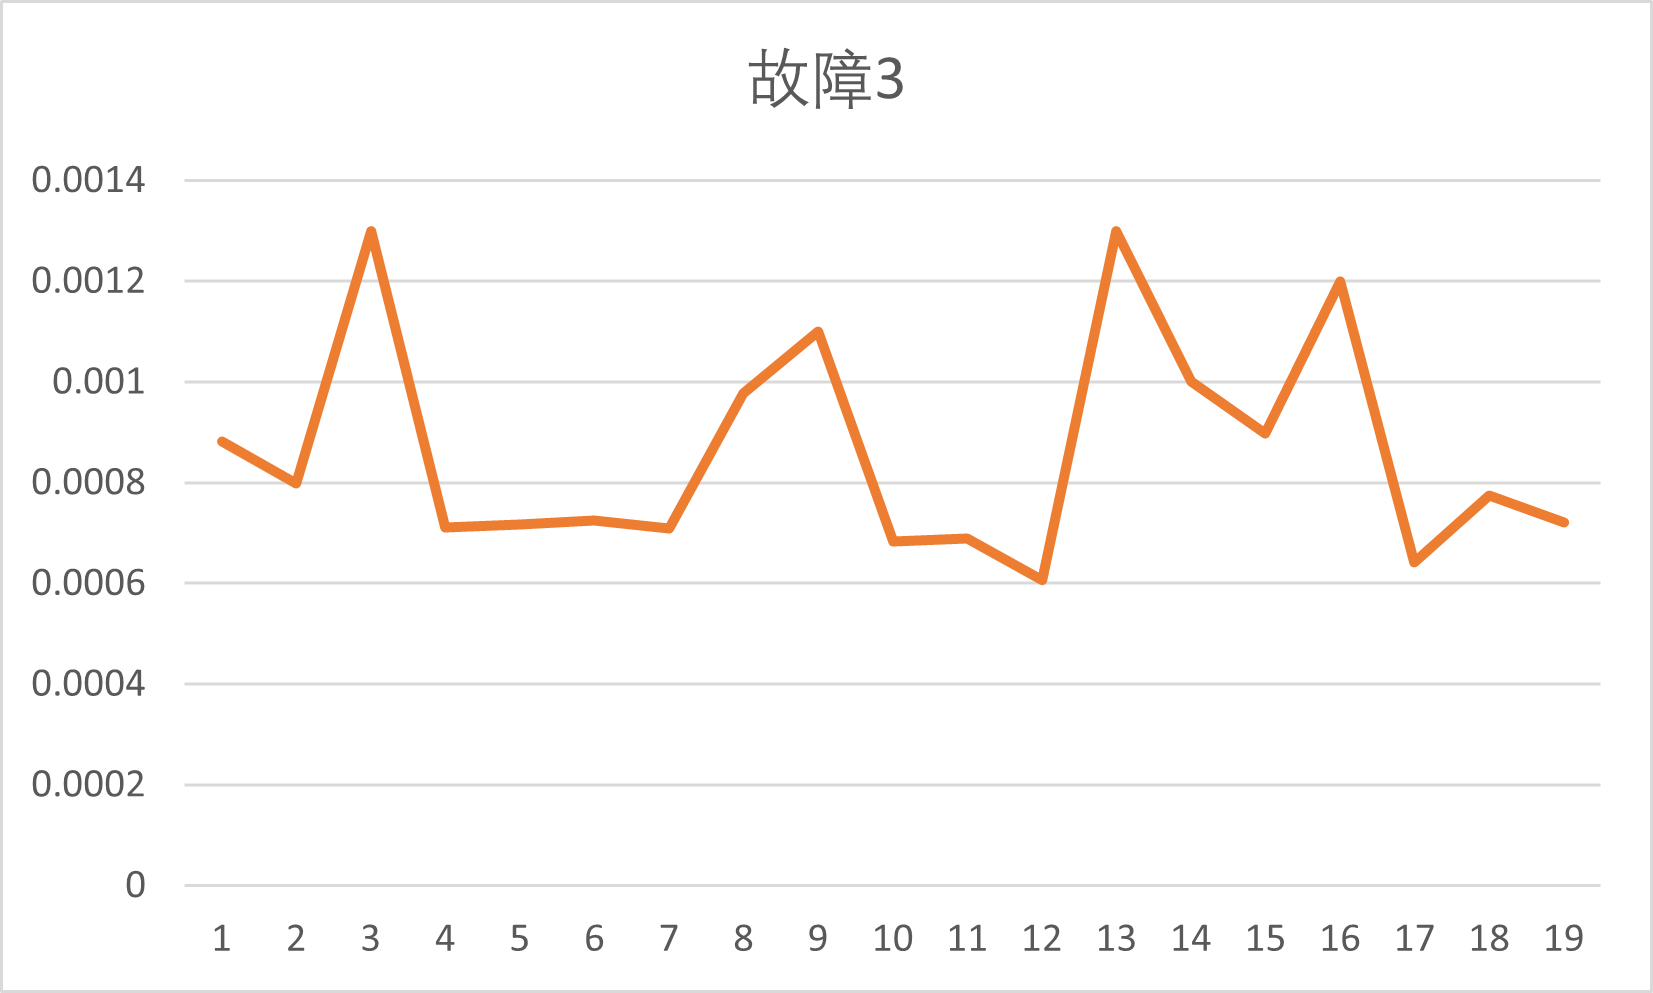
\includegraphics[width=0.45\textwidth]{exp5_4}}
	\subfigure[故障4]{
		\label{Fig.sub.4}
		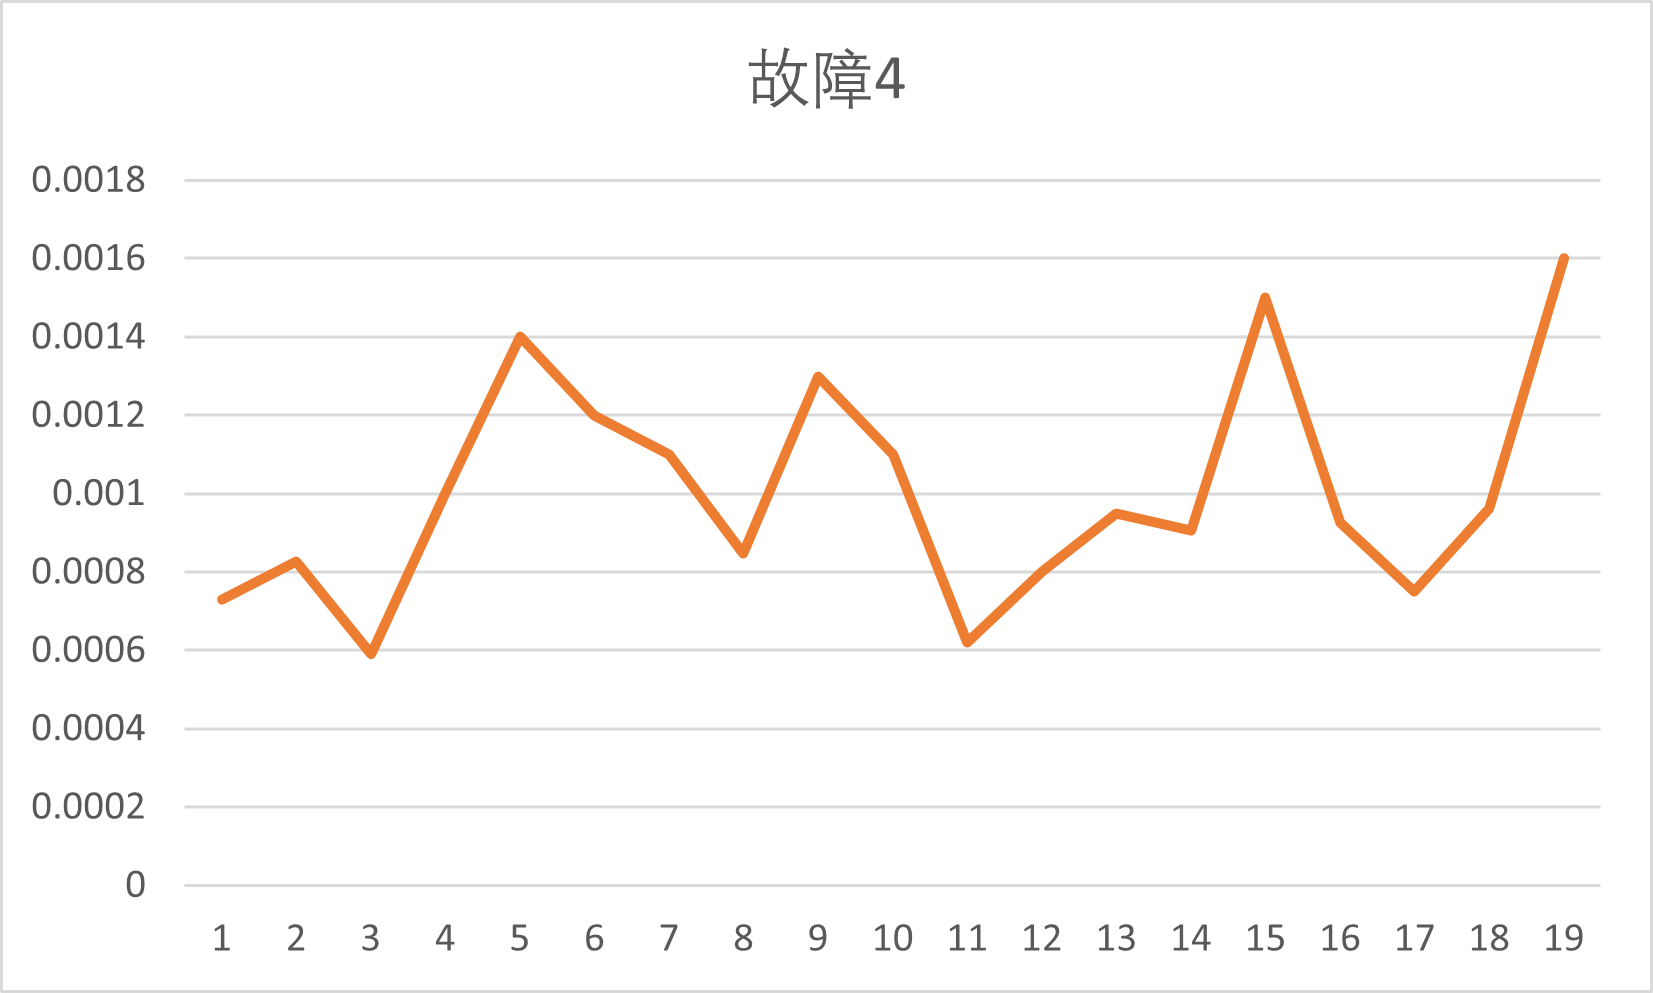
\includegraphics[width=0.45\textwidth]{exp5_5}}
	\caption{各故障的判别式的平均值}
	\label{Fig.main}
\end{figure}
% Please add the following required packages to your document preamble:
% \usepackage{booktabs}
\begin{table}[]
	\centering
	\begin{tabular}{ccccc}
		\hline
		& 故障1    & 故障2    & 故障3    & 故障4    \\ \hline
		$max$      & 0.0138 & 0.0017 & 0.0013 & 0.0016 \\
		$\Delta_a(1.5\times max)$ & 0.0207 & 0.0026 & 0.0020 & 0.0024 \\ \hline
	\end{tabular}
\end{table}
得到各个故障的$\Delta_\alpha$之后,再进行新故障的辨识。新故障由正常工况数据代替,效果如下:
\begin{figure}[H] %H为当前位置,!htb为忽略美学标准,htbp为浮动图形
	\centering %图片居中
	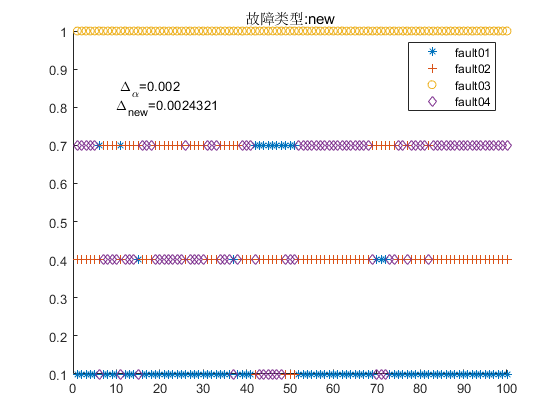
\includegraphics[width=1.0\textwidth]{exp5_6} %插入图片,[]中设置图片大小,{}中是图片文件名
	\caption{新型故障的测试} %最终文档中希望显示的图片标题
	\label{Fig.main2} %用于文内引用的标签
\end{figure}
\begin{shaded}
	注意:判别式的临界值$\Delta_{new}$可以选择大一点,这样可以尽量保证属于故障库的数据不被认为是新故障(灵敏度要低一些),可以选择小一点,这样可以尽量保证属于新型故障被认出来。
\end{shaded}
\begin{figure}[H] %H为当前位置,!htb为忽略美学标准,htbp为浮动图形
	\centering %图片居中
	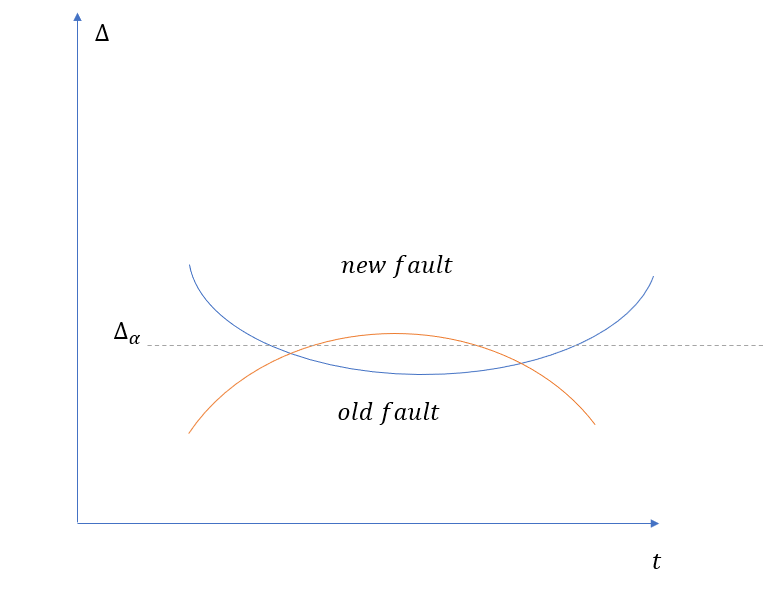
\includegraphics[width=1.0\textwidth]{newfault} %插入图片,[]中设置图片大小,{}中是图片文件名
	\caption{合适的$\Delta_{\alpha}$} %最终文档中希望显示的图片标题
	\label{Fig.main2} %用于文内引用的标签
\end{figure}
\subsection{附加实验}
本次实验主要讨论一些极端情况下算法是否有效。
\subsubsection{加入正常数据}
前面的实验都没有将正常数据加进来,这次考虑将正常工况的数据加进来。
\begin{figure}[H]
	\centering  %图片全局居中
	\subfigure[故障1]{
		\label{Fig.sub.1}
		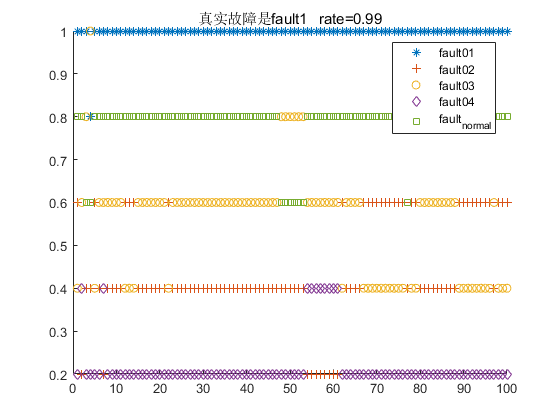
\includegraphics[width=0.45\textwidth]{exp6_1}}
	\subfigure[故障2]{
		\label{Fig.sub.2}
		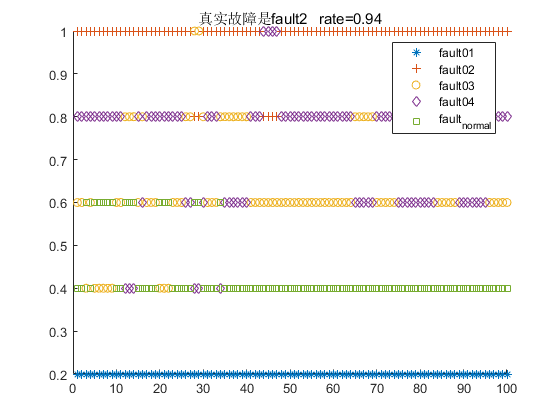
\includegraphics[width=0.45\textwidth]{exp6_2}}
	\subfigure[故障3]{
		\label{Fig.sub.3}
		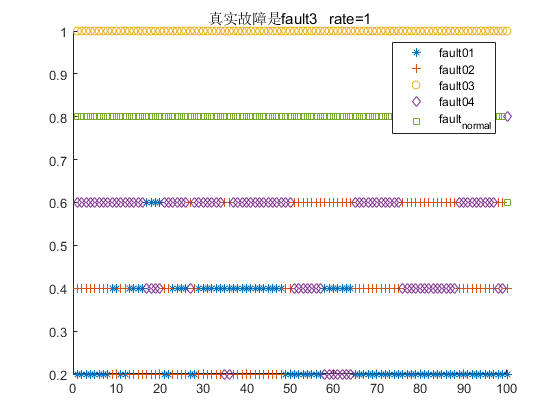
\includegraphics[width=0.45\textwidth]{exp6_3}}
	\subfigure[故障4]{
		\label{Fig.sub.4}
		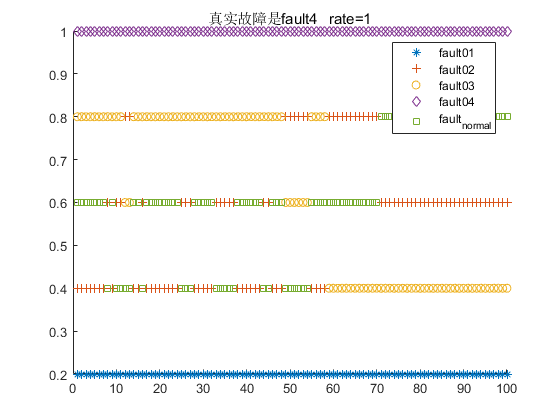
\includegraphics[width=0.45\textwidth]{exp6_4}}
	\subfigure[故障5]{
		\label{Fig.sub.4}
		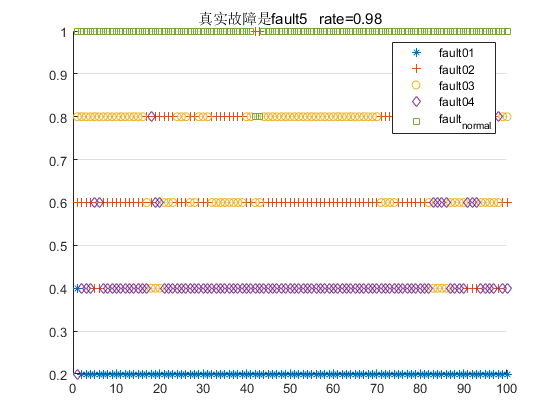
\includegraphics[width=0.45\textwidth]{exp6_5}}
	\caption{加入正常工况数据}
	\label{Fig.main}
\end{figure}
\subsubsection{$\ldots$}
$\mu$
\end{document}
